% !TEX TS-program = lualatex
%---------%---------%---------%---------%---------%---------%---------%---------
%  First version created by Alain Matthes le 2012-02-22.
%  Copyright (C) 2020 Alain Matthes 
% This file may be distributed and/or modified
%
% 1. under the LaTeX Project Public License , either version 1.3
% of this license or (at your option) any later version and/or
% 2. under the GNU Public License. 
%---------%---------%---------%---------%---------%---------%---------%---------
% Version 1.3 2024/08/14
\RequirePackage{luatex85}
\RequirePackage{silence}
\WarningsOff[latex]
\WarningsOff[latexfont]
\documentclass[a4paper,nofonts]{tufte-handout}
%---------%---------%---------%---------%---------%---------%---------%---------
\usepackage{fontspec}
\setmainfont{texgyrepagella}%
[ Extension = .otf ,
  UprightFont = *-regular,
  ItalicFont = *-italic,
  BoldFont = *-bold,
  BoldItalicFont = *-bolditalic,
  Ligatures=TeX,
  Numbers={Lowercase,Monospaced}]
\setsansfont{texgyreheros}%
[ Extension = .otf,
  UprightFont = *-regular ,
  ItalicFont  = *-italic  ,
  BoldFont    = *-bold    ,
  BoldItalicFont = *-bolditalic]
\setmonofont{lmmono10-regular.otf}%
[ Numbers={Lining,SlashedZero},
  ItalicFont=lmmonoslant10-regular.otf,
  BoldFont=lmmonolt10-bold.otf,
  BoldItalicFont=lmmonolt10-boldoblique.otf]
\newfontfamily\ttcondensed{lmmonoltcond10-regular.otf}
 %% (La)TeX font-related declarations:
\linespread{1.05}% Pagella needs more space between lines
\frenchspacing
%---------%---------%---------%---------%---------%---------%---------%---------
\usepackage[dvipsnames,svgnames]{xcolor}  
\usepackage{graphicx,rotating} 
\usepackage[object=vectorian]{pgfornament}
\usetikzlibrary{chains,
                calc,
                scopes,
                decorations,
                decorations.text,
                decorations.markings,
                positioning,
                shapes.geometric}
 
\usepackage{tkzexample,tikzrput,pict2e,picture} 

\usepackage{eso-pic,calc}
\usepackage{fancyvrb}
\usepackage{fourier}
\usepackage{amsmath,lipsum}  % extended mathematics
\usepackage{array,booktabs} % book-quality tables
\usepackage{multicol} % multiple column layout facilities
\usepackage[babel=true]{microtype}
\DisableLigatures{encoding = *, family = *}
\usepackage[english]{babel}   
\setkeys{Gin}{width=\linewidth,totalheight=\textheight,keepaspectratio}
\graphicspath{{graphics/}} % set of paths to search for images
%\geometry{showframe} % display margins for debugging page layout
\fvset{fontsize=\small}
\hypersetup{% 
pdfauthor = {Alain Matthes},
pdftitle = {pgfornament},
pdfsubject = {Documentation de pgfornament},
colorlinks=true,
linkcolor=orange,
urlcolor=orange} 

% section  (end) 
%---------%---------%---------%---------%---------%---------%---------%---------
\title{The Ornaments package}
\author{Alain Matthes}
\makeatletter
\AddToShipoutPicture{%
\begingroup 
\setlength{\@tempdima}{2mm}%
\setlength{\@tempdimb}{\paperwidth-\@tempdima-1cm}%
\setlength{\@tempdimc}{\paperheight-\@tempdima}%
\put(\LenToUnit{\@tempdima},\LenToUnit{\@tempdimc}){%
  \pgfornament[color=Maroon,anchor=north west,width=1cm]{39}}
\put(\LenToUnit{\@tempdimb},\LenToUnit{\@tempdimc}){%
  \pgfornament[color=Maroon,anchor=north east,width=1cm,symmetry=v]{39}} 
\put(\LenToUnit{\@tempdima},\LenToUnit{\@tempdima}){%
  \pgfornament[color=Maroon,anchor=south west,width=1cm,symmetry=h]{39}}
\put(\LenToUnit{\@tempdimb},\LenToUnit{\@tempdima}){%
  \pgfornament[color=Maroon,anchor=south east,width=1cm,symmetry=c]{39}}    
\endgroup  
} 
\let\strippt\strip@pt     
\makeatother
   
\newcommand{\eachpageornament}{%
\begin{picture}(0,0)
\put(0,0){\pgfornament[width=1cm]{41}};
\put(\strippt\textwidth,0){\pgfornament[width=1cm,symmetry=v]{41}};
\put(0,-\strippt\textheight){\pgfornament[width=1cm,symmetry=h]{41}};
\put(\strippt\textwidth,-\strippt\textheight){\pgfornament[width=1cm,symmetry=c]{41}};  %
\end{picture}}


% Standardize command font styles and environments
\newcommand{\docparen}[1]{\ensuremath{(#1)}}% optional command argument
\definecolor{fondpaille}{cmyk}{0,0,0.1,0}
\pagecolor{fondpaille}
\color{Maroon}
\colorlet{graphicbackground}{fondpaille}
\colorlet{numbackground}{fondpaille}
\colorlet{codebackground}{Periwinkle!10}
\colorlet{codeonlybackground}{Periwinkle!10}
\colorlet{textcodecolor}{MidnightBlue} % Maroon
\colorlet{numcolor}{gray}
\newcommand*{\tkzname}[1]{\textbf{\texttt{\textcolor{Maroon}{#1}}}}
\newcommand*{\PGF}{\tkzname{PGF}}
\newcommand*{\TIKZ}{\tkzname{Ti\emph{k}Z}}
\newcommand*{\pdf}{\textsc{pdf}}
\newcommand*{\pgfname}{\textsc{pgf}}
\newcommand*{\tikzname}{Ti\emph{k}Z}
\newcommand*{\pstricks}{\textsc{pstricks}}   %
\newcommand*{\tkzAttention}[3]{\ \\\llap{\textcolor{#3}{#1\hskip #2}}}
\newcommand*{\tkzHand}{\ \\\llap{\textcolor{red}{\lefthand\hskip1em}}}
\newcommand*{\tkzHandBomb}{\ \\\llap{\textcolor{red}{\lefthand\ \bomb\hskip1em}}}
\newcommand*{\tkzBomb}{\ \\\llap{\textcolor{red}{\bomb\hskip1em}}}
\newcommand*{\tkzTwoBomb}{\ \\\llap{\textcolor{red}{\bomb\ \bomb\hskip1em}}}
\newcommand*{\tkzimp}[1]{\textbf{#1}}
\newcommand*{\tkzcname}[1]{\textbf{\texttt{\textcolor{Maroon}{\textbackslash#1}}}}
\newcommand*{\tkzhname}[1]{\textbf{\texttt{\textcolor{Maroon}{\textbackslash#1}}}}
% Macros for typesetting the documentation
\newcommand{\hlred}[1]{\textcolor{Maroon}{#1}}% prints in red
\newcommand{\hangleft}[1]{\makebox[0pt][r]{#1}}
\newcommand{\hairsp}{\hspace{1pt}}% hair space
\newcommand{\hquad}{\hskip0.5em\relax}% half quad space
\newcommand{\TODO}{\textcolor{red}{\bf TODO!}\xspace}
\newcommand{\tuftebs}{\symbol{'134}}% a backslash in tt type in OT1/T1
\newcommand{\doccmdnoindex}[2][]{\texttt{\tuftebs#2}}% command name -- adds backslash automatically (and doesn't add cmd to the index)
\newcommand{\doccmddef}[2][]{%
  \hlred{\texttt{\tuftebs#2}}\label{cmd:#2}%
  \ifthenelse{\isempty{#1}}%
    {% add the command to the index
      \index{#2 command@\protect\hangleft{\texttt{\tuftebs}}\texttt{#2}}% command name
    }%
    {% add the command and package to the index
      \index{#2 command@\protect\hangleft{\texttt{\tuftebs}}\texttt{#2} (\texttt{#1} package)}% command name
      \index{#1 package@\texttt{#1} package}\index{packages!#1@\texttt{#1}}% package name
    }%
}% command name -- adds backslash automatically

\newcommand{\doccmd}[2][]{%
  \texttt{\tuftebs#2}%
  \ifthenelse{\isempty{#1}}%
    {% add the command to the index
      \index{#2 command@\protect\hangleft{\texttt{\tuftebs}}\texttt{#2}}% command name
    }%
    {% add the command and package to the index
      \index{#2 command@\protect\hangleft{\texttt{\tuftebs}}\texttt{#2} (\texttt{#1} package)}% command name
      \index{#1 package@\texttt{#1} package}\index{packages!#1@\texttt{#1}}% package name
    }%
}% command name -- adds backslash automatically
\newcommand{\docopt}[1]{\ensuremath{\protect\langle}\textrm{\textit{#1}}\ensuremath{\protect\rangle}}% optional command argument
\newcommand{\docarg}[1]{\textrm{\textit{#1}}}% (required) command argument
\newenvironment{docspec}{\begin{quotation}\ttfamily\parskip0pt\parindent0pt\ignorespaces}{\end{quotation}}% command specification environment
\newcommand{\docdist}[1]{\texttt{#1}\index{#1 distribution@\texttt{#1} distribution}\index{distributions!#1@\texttt{#1}}}% environment name
\newcommand{\docenv}[1]{\texttt{#1}\index{#1 environment@\texttt{#1} environment}\index{environments!#1@\texttt{#1}}}% environment name
\newcommand{\docenvdef}[1]{\hlred{\texttt{#1}}\label{env:#1}\index{#1 environment@\texttt{#1} environment}\index{environments!#1@\texttt{#1}}}% environment name
\newcommand{\docoption}[2]{\texttt{#1}\index{#1 option@\texttt{#1} option}\index{options(#2)!#1@\texttt{#1}}}% package name
\newcommand{\docpkg}[1]{\texttt{#1}\index{#1 package@\texttt{#1} package}\index{packages!#1@\texttt{#1}}}% package name
\newcommand{\doclib}[1]{\texttt{#1}\index{#1 tikz library@\texttt{#1} library}\index{library!#1@\texttt{#1}}}% libray name
\newcommand{\doccls}[1]{\texttt{#1}}% document class name
\newcommand{\docclsopt}[1]{\texttt{#1}\index{#1 class option@\texttt{#1} class option}\index{class options!#1@\texttt{#1}}}% document class option name
\newcommand{\docclsoptdef}[1]{\hlred{\texttt{#1}}\label{clsopt:#1}\index{#1 class option@\texttt{#1} class option}\index{class options!#1@\texttt{#1}}}% document class option name defined
\newcommand{\docmsg}[2]{\bigskip\begin{fullwidth}
\noindent\ttfamily#1\end{fullwidth}\medskip\par\noindent#2}
\newcommand{\docfilehook}[2]{\texttt{#1}\index{file hooks!#2}\index{#1@\texttt{#1}}}
\newcommand{\doccounter}[1]{\texttt{#1}\index{#1 counter@\texttt{#1} counter}}
\newcommand{\docStyle}[1]{\texttt{#1}\index{#1 style(\TIKZ)@\texttt{#1} style(\TIKZ)}\index{styles(\TIKZ)!#1@\texttt{#1}}}% package name
\newcommand*{\Imacro}[1]{\index{#1_1@\texttt{\textbackslash#1}}}%n
\newcommand{\docfamily}[1]{\texttt{#1}\index{#1 family@\texttt{#1} family}\index{families!#1@\texttt{#1}}}% package name
\newcommand{\docvo}[1]{\texttt{#1}\index{#1 vector ornament@\texttt{#1} vector ornament}\index{vector ornaments!#1@\texttt{#1}}}% package name
%


\endinput
\usepackage{makeidx}
\makeindex
\renewenvironment{theindex}
  {\renewcommand\item{\par\hangindent 40pt}
   \renewcommand\subitem{\item\hspace*{20pt}}
   \renewcommand\subsubitem{\item\hspace*{30pt}}
   \renewcommand\indexspace{\par \vskip 10pt plus 5pt minus 3pt\relax}
   \section{\indexname}
   \begin{multicols}{2}%
    \parindent=0pt
     \small%
      }
  {\end{multicols}%
  }
  
\makeatletter 
\newcommand{\getpgfornamentDim}[1]{%
 {\@pgfornamentDim{#1}%
 X:~\@pgfornamentX\\Y:~\@pgfornamentY}%
}
\newcommand{\adjustpgfornamentDim}[1]{%
\@pgfornamentDim{#1}%
\pgfmathsetmacro{\pgfcoeff}{\@pgfornamentX/\@pgfornamentY}%
}
\makeatother

\newcommand{\ornamentview}[1]{%
\foreach \n in {#1} {%
\begin{tikzpicture}
  \adjustpgfornamentDim{\n}
  \ifdim\pgfcoeff pt >1 pt \relax \def\adjustXY{2}
  \else
  \pgfmathsetmacro{\adjustXY}{2*\pgfcoeff}
  \fi 
\draw[Maroon](-1.25cm,-1.25cm) rectangle (1.25cm,1.25cm);
\node[inner sep=0pt] (element) {\pgfornament[width=\adjustXY cm]{\n}};
\node[anchor=north west,inner sep=0pt,font=\small\bfseries\sffamily,color=red] at (2.05cm,1.05cm) {\n};
\node[anchor=west,text width=4em,font=\footnotesize] at (1.85cm,0) {\getpgfornamentDim{\n}};
\end{tikzpicture}%
\space\space\space\space}}%

%---------%---------%---------%---------%---------%---------%---------%---------
%---------%---------%---------%---------%---------%---------%---------%---------
\begin{document}

\maketitle
\noindent\pgfornament[symmetry=c,width=2cm]{46}
\begin{marginfigure}
  
\begin{tikzpicture}[baseline={(current bounding box.center)}] \tikzset{pgfornamentstyle/.style={
  draw=Goldenrod,fill=Red,line width=1pt}} 
  \node[fill=black,circle,draw=Red,line width=2pt,inner sep=8pt]
  at (0,0) {\pgfornament[scale=0.38]{56}}; 
  \end{tikzpicture}
\end{marginfigure}


\bigskip
\noindent\pgfornament[width=0.75 cm]{152}\ (Version  1.3 2024/08/14)
\begin{abstract}

This document describes the \LaTeX\ package \emph{\docpkg{pgfornament}} and presents the syntax and parameters of the macro "pgfornament".
It also provides examples and comments on the package's use.

 Firstly, I would like to thank {Till \textsc{Tantau}} for the  beautiful \LaTeX\ package, namely \TIKZ.

I am grateful to  Vincent \textsc{Le Moign} for allowing us to distribute the ornaments \sidenote{ \url{http://www.vectorian.net/} (free sample)} in the format Pstricks and \PGF/\TIKZ.

I also thank \textsc{P. Fradin} who first created a package on ornaments in relation to PStricks, which gave me the idea to do the same thing in relation to \TIKZ.

I would like to thank also {Enrico  \textsc{Gregorio}} for some great ideas used in this package. You will find at the end of this document the 196 symbols provided with the package.

With this new version comes a new family of ornaments.
\textsc{Chennan Zhang} drew the motifs using a CAD application, re-drew them in TikZ, and granted permission for these to be turned into a library (\emph{\docpkg{pgfornament-han}}) suitable for use with the pgfornament package by \textsc{LianTze Lim}.
It is now possible to use directly the library for Chinese traditional motifs and patterns.

Next to the document you are reading, you will find documentation on the package \emph{\docpkg{tikzrput}}.
\end{abstract}

%---------%---------%---------%---------%---------%---------%---------%---------
\vspace{1cm}
\hfil  \pgfornament[width=4cm]{84}\hfil

\tableofcontents

\vspace{1cm}
\hfil  \pgfornament[width=4cm]{84}\hfil

\listoffigures

\vspace{1cm}
\hfil  \pgfornament[width=4cm]{84}\hfil

\section{How to install the package}
\label{sec:how_to_install}
With \docdist{TeXLive}, if you need to install it by yourself, a TDS compliant zip archive is
provided (pgfornament.zip).  Just download that file, and unpack it in
your TDS directory (~/texmf for Unix-like systems).
\begin{itemize}
  \item \docpkg{pgfornament}  must to be in \texttt{~/texmf/tex/latex}
  \item pgflibraryvectorian.code.tex must to be in \texttt{~/texmf/tex/latex}
  \item pgflibraryhan.code.tex must to be in \texttt{~/texmf/tex/latex}
  \item pgflibraryam.code.tex must to be in \texttt{~/texmf/tex/latex}
  \item the folder vectorian must to be in \texttt{~/texmf/tex/generic}
  \item the folder han must to be in \texttt{~/texmf/tex/generic}
  \item the folder am must to be in \texttt{~/texmf/tex/generic}
\end{itemize}

With \docdist{MiKTeX}, copy the folder {\color{black}\texttt{pgfornament}} into \verb+C:\texmf\tex\latex+, then
run {\color{red}\texttt{MiKTeX Options}}  . In the {\color{black}\texttt{File name database}}  section, click on  {\color{red}\texttt{Refresh now}}.

\section{How to use the package}
\label{sec:how_to_use}
You only need to add \\
{\color{black}\verb+\usepackage{pgfornament}+} \\ or  \\{\color{black}\verb+\usepackage[object=vectorian]{pgfornament}+}\\
 in your preamble. The  pgfornament package loads \TIKZ.

 Without any options, pgfornament package uses the \docfamily{vectorian} symbols. If you want to use other symbols, you give the name of the list of symbols like this : \\
{\color{black}\verb+\usepackage[object=pgfhan]{pgfornament}+}.\\
"\docfamily{pgfhan}" is the family for Chinese traditional motifs and patterns.

 I create \docfamily{am}  to show you how to create new symbols and how to use it (see the section \ref{am1def}).
 You can see below, the minimum code to get a vector ornament.
\colorlet{graphicbackground}{blue!10!white}%
\colorlet{codebackground}{red!10}%

\begin{marginfigure}%
\begin{center}
  \pgfornament[width = 2cm,
               color = red]{1}
\end{center}
\caption{Result of the minimal code}
\end{marginfigure}

\begin{tkzexample}[code only,very small]
 \documentclass{scrartcl}
 \usepackage{pgfornament}
 \begin{document}
 \pgfornament[width = 2cm,
              color = red]{1}
 \end{document}
\end{tkzexample}

If you want to work with the Han library

\newpgfornamentfamily{pgfhan}
\begin{marginfigure}%
\begin{center}
  \pgfornament[width = 2cm,
               color = SeaGreen]{78}
\end{center}
\caption{Result of the minimal code}
\end{marginfigure}

\begin{tkzexample}[code only,very small]
 \documentclass{scrartcl}
 \usepackage[object=pgfhan]{pgfornament}
 \begin{document}
 \pgfornament[width = 2cm,
              color = SeaGreen]{78}
 \end{document}
\end{tkzexample}
\newpgfornamentfamily{vectorian}

How to use different families of ornaments?

You have two possibilities: the macro \doccmd{newpgfornamentfamily} or 
an environment \docenv{newfamily}

For example:
\newpgfornamentfamily{pgfhan}
\pgfornament[width = 2cm, color = SeaGreen]{59}
\newpgfornamentfamily{vectorian}
\pgfornament[width = 2cm, color = SeaGreen]{59}

with the code:
\begin{tkzexample}[code only, very small]
  \newpgfornamentfamily{pgfhan}
  \pgfornament[width = 2cm, color = SeaGreen]{59}
  \newpgfornamentfamily{vectorian}
  \pgfornament[width = 2cm, color = SeaGreen]{59}
\end{tkzexample}

Now with the environment. At the end, you will find the previous ornament library.

\begin{newfamily}[pgfhan]
  
\begin{tikzpicture}
  \node{ \pgfornament[color=Dandelion,width=2cm]{1}};
  \end{tikzpicture}
\end{newfamily}


\begin{tikzpicture}
\node{\pgfornament[color=MidnightBlue,width=2cm]{1}};
\end{tikzpicture}

with the code:
\begin{tkzexample}[code only, very small]
\begin{newfamily}[pgfhan]
  
\begin{tikzpicture}
  \node{ \pgfornament[color=Dandelion,width=2cm]{1}};
  \end{tikzpicture}
\end{newfamily}


\begin{tikzpicture}
\node{\pgfornament[color=MidnightBlue,width=2cm]{1}};
\end{tikzpicture}
\end{tkzexample}  
  
\section{The main macro}
\label{sec:the_main_macro}

The macro \doccmd{pgfornament} draws the object  linked to  the given number, with the vectorian family this number is between  $1$ and now $196$. This macro can be used alone, or inside a picture. It's defined by an environment \emph{\docenv{tikzpicture}} placed at the current point.

The objects displayed depend of the option used when \doccmd{pgfornament} is called.
The specifications of the {\color{red}\Verb|\pgfornament|} command is:
\begin{docspec}
 \color{black} \doccmd{pgfornament[\docopt{options}]\{\docarg{number}\}}
\end{docspec}

The result is a picture defined by a \emph{\docenv{tikzpicture}} environment.

\subsection{Number argument}
\label{sub:arg_number}

The number designs an object of a list by a rank.
\begin{marginfigure}
\begin{center}
  \pgfornament[width=2cm,color=RubineRed]{1}
\end{center}
\caption{Vectorian ornament n° 1}
\end{marginfigure}
\begin{tkzexample}[code only,width=5cm,very small]
  \usepackage{pgfornament}
  ...
  \pgfornament[width=2cm]{1}
\end{tkzexample}

\medskip
\begin{marginfigure}
\begin{center}
  \pgfornament[width=2cm,color=SeaGreen]{2}
\end{center}
  \caption{Vectorian ornament n° 2}
\end{marginfigure}
\begin{tkzexample}[code only,width=5cm,very small]
  \usepackage{pgfornament}
  ...
  \pgfornament[width=2cm]{2}
\end{tkzexample}

\medskip
\begin{marginfigure}
\begin{center}
\begin{newfamily}[pgfhan]

\begin{tikzpicture}
 \node {\pgfornament[color=red,width=2cm]{57}};
\end{tikzpicture}
\end{newfamily}
\end{center}
\caption{Chinese ornament n° 57}
\end{marginfigure}
\begin{tkzexample}[code only,width=5cm,very small]
  \usepackage[object=pgfhan]{pgfornament}
    ...
  \pgfornament[color=Mahogany,width=2cm]{57}
\end{tkzexample}

\medskip
\begin{tkzexample}[code only,width=5cm,very small]
  \usepackage[object=am]{pgfornament}
   ...
  \pgfornament[width=4cm]{1}
\end{tkzexample}
\begin{marginfigure}
\begin{newfamily}[am]

\begin{tikzpicture}
 \pgfornament[color=Dandelion,width=2cm]{1}
\end{tikzpicture}
\end{newfamily}
\newpgfornamentfamily{vectorian}
  \caption{am ornament n° 1}
\end{marginfigure}

\subsection{Argument and  options}
\label{sub:the_options}
The macro has  six options. You have four possibilities for the last option \Verb+symmetry+.
The next table describes these options.

\begin{table}[h]\index{pgfornament!options}
{ \small   \begin{tabular}{lll}
      \toprule
 name & default  &  definition \\
\midrule
\docoption{scale}{pgfornament}         & 1     & ratio of height to width is unchanged\\
\docoption{width}{pgfornament}         & \{\}  & set the width, ratio unchanged  \\
\docoption{height}{pgfornament}        & \{\}  & set the height, ratio unchanged \\
\docoption{color}{pgfornament}         & black & color of the ornament  \\
\docoption{opacity}{pgfornament}       & 1     & nb inf 1, opacity of the ornament  \\
\docoption{ydelta}{pgfornament}        & 0 pt  & value to adjust vertically the ornament  \\
\docoption{symmetry=v}{pgfornament}    & none  &  vertical symmetry\\
\docoption{symmetry=h}{pgfornament}    & none  & horizontal symmetry \\
\docoption{symmetry=c}{pgfornament}    & none  & central symmetry \\
\docoption{symmetry=none}{pgfornament} & none  & no  symmetry by default \\
\bottomrule
\end{tabular} }
\caption{List of  options for the pgfornament macro.}
  \label{tab:pgfornament-options}
\end{table}

\subsection{Examples of the use of options}
\label{sub:examples}
\begin{enumerate}\setlength{\itemsep}{30pt}
\item Option \docoption{scale}{pgfornament}
\begin{tkzexample}[code only,very small]
  \pgfornament[scale=0.25]{77}
\end{tkzexample}
\begin{marginfigure}
  \pgfornament[scale=0.25]{77}
\caption{Option \tkzname{scale}}
\end{marginfigure}
\item Option \docoption{width}{pgfornament}
\begin{tkzexample}[code only,very small]
 \pgfornament[width=5cm]{77}
\end{tkzexample}
\begin{marginfigure}
  \pgfornament[width=5cm]{77}
\caption{Option \tkzname{width}}
\end{marginfigure}
\item Option \docoption{height}{pgfornament}
\begin{tkzexample}[code only,very small]
\pgfornament[height=1cm]{77}
\end{tkzexample}
\begin{marginfigure}
  \pgfornament[height=1cm]{77}
\caption{Option \tkzname{height}}
\end{marginfigure}

\item Option \docoption{color}{pgfornament}
\begin{tkzexample}[code only,very small]
\pgfornament[height=1cm,color=green!20!black]{77}
\end{tkzexample}
\begin{marginfigure}
\pgfornament[height=1cm,color=green!20!black]{77}
\caption{Option \tkzname{color}}
\end{marginfigure}


\begin{marginfigure}
  \pgfornament[color=MidnightBlue,width=3cm]{24}%
  \caption{How to use \tkzname{color}}
\end{marginfigure}
\begin{tkzexample}[code only,very small]
  \pgfornament[color=MidnightBlue,width=3cm]{24}%
\end{tkzexample}

\item Option \docoption{opacity}{pgfornament}
\begin{tkzexample}[code only,very small]
\pgfornament[height=1cm,color=green!20!black,opacity=0.2]{77}
\end{tkzexample}
\begin{marginfigure}
\pgfornament[height=1cm,color=green!20!black,opacity=0.2]{77}
\caption{Option \tkzname{opacity}}
\end{marginfigure}

\begin{marginfigure}
  \pgfornament[width=5cm]{2}
      \caption{Example for symmetry}
\end{marginfigure}

\item Option \docoption{symmetry=h}{pgfornament} 
(Symmetry  horizontal  axis)
\begin{marginfigure}
 \tikzset{pgfornamentstyle/.style={draw=BlueGreen,
             fill=BlueGreen!20,fill opacity=.5,thick}}%
\pgfornament[width=5cm,symmetry=h]{2}
\caption{Horizontal symmetry}
\end{marginfigure}


\item Option \docoption{symmetry=v}{pgfornament}
(Symmetry  vertical axis)
\begin{marginfigure}
\tikzset{pgfornamentstyle/.style={draw=MidnightBlue,
        fill=MidnightBlue!20,fill opacity=.5,thick}}%
\pgfornament[width=5cm,symmetry=v]{2}
\caption{Vertical symmetry}
\end{marginfigure}

\item Option \docoption{symmetry=c}{pgfornament}
(Symmetry with respect to the origin)
\begin{marginfigure}
\tikzset{pgfornamentstyle/.style={draw=RubineRed,
           fill=RubineRed!20,fill opacity=.5,thick}}%
\pgfornament[width=5cm,symmetry=c]{2}%
\caption{Central symmetry}
\end{marginfigure}

\item Option \docoption{ydelta}{pgfornament}

\begin{marginfigure}%
\pgfornament[color=MidnightBlue,width=1cm,ydelta=-10pt]{25}%
\pgfornament[color=PineGreen,width=1cm]{25}%
\pgfornament[color=Periwinkle,width=1cm,ydelta=+10pt]{25}%
\caption{How to use \tkzname{ydelta}}
\end{marginfigure}
\begin{tkzexample}[code only,very small]
  \pgfornament[color=MidnightBlue,width=2cm,ydelta=-10pt]{25}%
  \pgfornament[color=PineGreen,width=2cm]{25}%
  \pgfornament[color=Periwinkle,width=2cm,ydelta=+10pt]{25}%
\end{tkzexample}
\end{enumerate}

\clearpage\newpage
\subsection{Style \docStyle{pgfornamentstyle}}
\label{sub:pgfornamentstyle}
This style can modify some options like the color and also how to fill the symbol when it's possible.
\begin{marginfigure}%

\begin{tikzpicture}
  \tikzset{pgfornamentstyle/.style={
           fill=SpringGreen,
           fill opacity=.5,
           line width=1pt}}%
  \pgfornament[color=OliveGreen,scale=1.25,anchor=south]{24}%
\end{tikzpicture}
\caption{How to use the style \tkzname{pgfornamentstyle}}
\end{marginfigure}
\begin{tkzexample}[code only,very small]

\begin{tikzpicture}
  \tikzset{pgfornamentstyle/.style={
           fill=SpringGreen,
           fill opacity=.5,
           line width=1pt}}%
  \pgfornament[color=OliveGreen,scale=1.25,anchor=south]{24}%
\end{tikzpicture}
\end{tkzexample}

\subsection{Advanced options from \docpkg{\TIKZ}}
\label{sub:advanced_options}
\begin{marginfigure}

\begin{tikzpicture}
 \tikzset{pgfornamentstyle/.style={draw=Periwinkle,
             fill=SpringGreen}}%
 \node[draw=Periwinkle,circle,anchor=center,
      inner sep=0pt,fill=GreenYellow] at (0,0){%
\pgfornament[anchor=center]{24}};
\end{tikzpicture}
\caption{How to add \TIKZ ' styles}
\end{marginfigure}
\begin{tkzexample}[code only,very small]

\begin{tikzpicture}
 \tikzset{pgfornamentstyle/.style={draw=Periwinkle,
             fill=SpringGreen}}%
 \node[draw=Periwinkle,circle,anchor=center,
      inner sep=0pt,fill=GreenYellow] at (0,0){%
 \pgfornament[anchor=center]{24}};
\end{tikzpicture}
\end{tkzexample}

\section{What is a (pgf)ornament?}
\label{sec:what_is_a_pgf_ornament}
When you write  in your document \Verb|\pgfornament{1}|, you get the first ornament of a family (by default \docfamily{vectorian}'s family). This ornament is a vector object defined by an environment  \emph{\docenv{tikzpicture}}.
\begin{tkzexample}[code only,very small]
\begin{tikzpicture}[baseline={([yshift=\pgfornamentydelta]%
  current bounding box.\pgfornamentanchor)},pgfornamentstyle]
  \pgftransformscale{\pgfornamentscale}%
  \pgf@@ornament{#2}%
\end{tikzpicture}%
\end{tkzexample}

\medskip
You can modify the aspect of the picture if you change

 \doccmd{pgfornamentscale}, or \docStyle{pgfornamentstyle}. With  \doccmd{pgfornamentydelta}, or \doccmd{pgfornamentanchor}, you can move the picture but  this depends on the different environments. The next code gives the picture \ref{fig:minimum}. I chose this method so that the use is as simple as possible.
\begin{marginfigure}
 \pgfornament[anchor=center,scale=1]{1}
 \caption{Minimal code to get an ornament}
 \label{fig:minimum}
\end{marginfigure}
\begin{tkzexample}[code only,very small]
 \documentclass{scrartcl}
 \usepackage{pgfornament}
 \begin{document}
 \pgfornament{1}
 \end{document}
\end{tkzexample}

\medskip
The ornament is placed in a rectangle\sidenote{You can find the dimensions of this shape in the file pgflibraryvectorian.code.tex. The name of this file depends of the name of the vector family By default actually it's \docfamily{vectorian}.}.

\medskip
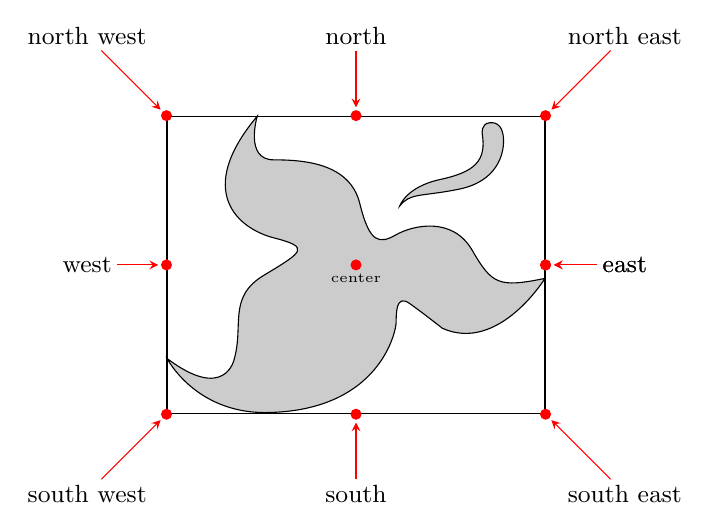
\begin{tikzpicture}[every node/.style={inner sep=0pt}]
  \tikzset{image/.style={circle,
                         fill=red,
                         minimum size = 4pt,
                         inner sep    = 0pt,
                         outer sep    = 1pt}
                         }

\node[inner sep = 1cm] (wrapper){\tikz
\node[draw](image) {\pgfsetfillopacity{0.2}\pgfornament{1}};};

\foreach \ancre  in {north,north east,east,south east,south,south west,west,north west,east}
{%
 \node [image] (i\ancre) at (image.\ancre) {};
 \node [outer sep=2pt] (w\ancre) at (wrapper.\ancre) {\small\ancre};
 \draw [red,->,>=stealth] (w\ancre)--(i\ancre);
 }
 \node[image,label=below:{\tiny center}] at (wrapper.center) {};
\end{tikzpicture}

On the last figure, I represent all the anchors \index{anchors} that you can use.  Now you will see how to place this picture on a page, in the flow of text or inside a complex picture.

\section{Placing a vector ornament on a page}
\label{sec:placement_on_a_page}

\unitlength=1pt
\noindent\eachpageornament
\subsection{On each page with the package \docpkg{eso-pic}}
\label{sub:with_the_package_eso_pic}

You may have noticed the existence of an ornament placed at each corner of the pages. The next code explains how to do this. The only part of the code  linked to \docpkg{pgfornament} is to use the macro \doccmd{pgfornament}. To put the object at the right place on the page, we need to consider its width.

Perhaps you saw the ornaments in each corner of each page

I used the package \docpkg{eso-pic} and the next code. The macro \doccmd{put} places the ornament at a point but you need to change correctly the anchor.

\begin{tkzexample}[code only,very small]
\usepackage{eso-pic}
\makeatletter
\AddToShipoutPicture{%
\begingroup
\setlength{\@tempdima}{2mm}%
\setlength{\@tempdimb}{\paperwidth-\@tempdima-2cm}%
\setlength{\@tempdimc}{\paperheight-\@tempdima}%
\put(\LenToUnit{\@tempdima},\LenToUnit{\@tempdimc}){%
 \pgfornament[anchor=north west,width=2cm]{63}}
\put(\LenToUnit{\@tempdima},\LenToUnit{\@tempdima}){%
  \pgfornament[anchor=south west,width=2cm,symmetry=h]{63}}
\put(\LenToUnit{\@tempdimb},\LenToUnit{\@tempdimc}){%
  \pgfornament[anchor=north east,width=2cm,symmetry=v]{63}}
\put(\LenToUnit{\@tempdimb},\LenToUnit{\@tempdima}){%
  \pgfornament[anchor=south east,width=2cm,symmetry=c]{63}}
\endgroup
}
\makeatother
\end{tkzexample}
\Imacro{AddToShipoutPicture}  \Imacro{LenToUnit}  \Imacro{anchor}

\subsection{On one page with the picture environment}
\label{sub:with_the_picture_environment}

The next code is used to delimit the text area on the page defined by the tufte class.
\sidenote{\tkzcname{strippt} is defined by \tkzcname{let}\doccmd{strippt}\doccmd{strip@pt}}
\begin{tkzexample}[code only,very small]
\newcommand{\eachpageornament}{%
\unitlength=1pt
\begin{picture}(0,0)%
\put(0,0){\pgfornament[width=1cm]{41}};%
\put(\strippt\textwidth,0){%
     \pgfornament[width=1cm,symmetry=v]{41}};%
\put(0,-\strippt\textheight){%
      \pgfornament[width=1cm,symmetry=h]{41}};%
\put(\strippt\textwidth,-\strippt\textheight){%
      \pgfornament[width=1cm,symmetry=c]{41}};%
\end{picture}}%

\eachpageornament
\end{tkzexample}

\subsection{With \docpkg{\TIKZ}[\tkzname{remember picture},\tkzname{overlay}]}
\label{sub:with_tikz}

You can without \docpkg{eso-pic} but with \docpkg{\TIKZ}\  get the same result  on one page with the next macro.  \tkzname{remember picture}  is obligatory, this option tells \TIKZ\  that it should attempt to remember the position of the current picture on the page, you need to compile twice if you use such code. The option  \tkzname{overlay}\index{overlay}\ switches the computation of the bounding box so the pictures are not in the flow of the text and they don't modify the layout.

\begin{tkzexample}[code only,very small]
\newcommand{\eachpageornament}{%
\begin{tikzpicture}[remember picture, overlay]
    \node[anchor=north west] at (current page.north west){%
                      \pgfornament[width=2cm]{63}};
    \node[anchor=north east] at (current page.north east){%
                      \pgfornament[width=2cm,symmetry=v]{63}};
    \node[anchor=south west] at (current page.south west){%
                     \pgfornament[width=2cm,symmetry=h]{63}};
    \node[anchor=south east] at (current page.south east){%
                      \pgfornament[width=2cm,symmetry=c]{63}};
\end{tikzpicture}
}
\end{tkzexample}
\index{current page}

\section{Placing a vector ornament in the flow}
\label{sec:placing-ornament}
\subsection{\protect\pgfornament[anchor=south,width=1cm]{78}\  Directly\  \protect\pgfornament[anchor=south,width=1cm,symmetry=v]{78}}
\label{sub:directly}

The next code show you the effect of different choice of anchor.
\setlength{\fboxsep}{0pt}

{\color{black}baseline
\pgfsetfillopacity{0.2}%
\fbox{\pgfornament[anchor=south,width=2cm]{69}}%
\fbox{\pgfornament[width=2cm]{69}}%
\fbox{\pgfornament[anchor=north,width=2cm]{69}}%
\pgfsetfillopacity{1} baseline }

\begin{tkzexample}[code only,very small]
{ \color{black}baseline \pgfsetfillopacity{0.2}%
  \fbox{\pgfornament[anchor=south,width=2cm]{69}}%
  \fbox{\pgfornament[width=2cm]{69}}%
  \fbox{\pgfornament[anchor=north,width=2cm]{69}}%
  \pgfsetfillopacity{1} baseline }
\end{tkzexample}

\medskip
\noindent Perhaps you are interesting by the code to modify the subsection?

\begin{tkzexample}[code only,very small]
\subsection{\protect\pgfornament[anchor=south,width=1cm]{78}\
    Directly \
    \protect\pgfornament[anchor=south,width=1cm,symmetry=v]{78}}
\end{tkzexample}

\subsection{In the flow with \TIKZ}
\label{sub:in_the_flow_with_tikz}

\medskip
Generally, the best way is to place the ornament inside a node and the node inside  an environment \emph{tikzpicture}. You can need to specify the position of the node inside the \emph{\docenv{tikzpicture}} and you can add an anchor to place exactly the ornament like you want.

\begin{marginfigure}
  \begin{center}
    
\begin{tikzpicture}
      \foreach \a in {0,45,...,315}
     \node[anchor=west,rotate=\a,inner sep=0pt,xshift=12pt] {%
     \pgfornament[width=1cm]{88}};
    \end{tikzpicture}
  \end{center}
  \caption{Assembling of ornaments version 2}
\end{marginfigure}

\begin{tkzexample}[code only,very small]

\begin{tikzpicture}
    \foreach \a in {0,45,...,315}
      \node[anchor=west,rotate=\a,inner sep=0pt,xshift=12pt] {%
      \pgfornament[width=1cm]{88}};
\end{tikzpicture}
\end{tkzexample}

\begin{marginfigure}
  \begin{center}
    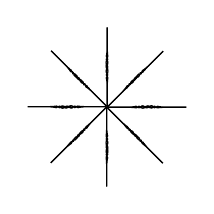
\begin{tikzpicture}
      \foreach \a in {0,45,...,315}
        \node[anchor=west,rotate=\a,inner sep=0pt] {%
     \pgfornament[width=1cm]{88}};
    \end{tikzpicture}
  \end{center}
  \caption{Assembling of ornaments version 1}
\end{marginfigure}

\begin{tkzexample}[code only,very small]
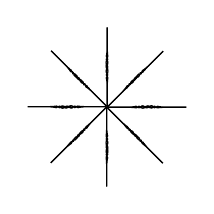
\begin{tikzpicture}
    \foreach \a in {0,45,...,315}
      \node[anchor=west,rotate=\a,inner sep=0pt] {%
      \pgfornament[width=1cm]{88}};
\end{tikzpicture}
\end{tkzexample}

\medskip
\emph{Remark :  It's difficult to get the same result with \emph{\doccmd{put}} and \emph{\doccmd{rotatebox}} but it's easy with the \emph{\docpkg{rotating}} package.}

\begin{marginfigure}
  \begin{center}
\foreach \a in {0,45,...,315}{%
   \turnbox{\a}{\pgfornament[width=1cm]{88}}}%
  \end{center}
\end{marginfigure}

\begin{tkzexample}[code only,very small]
  \foreach \a in {0,45,...,315}{%
     \turnbox{\a}{\pgfornament[width=1cm]{88}}}%
\end{tkzexample}

\section{Ornament inside a node}
\label{sec:inside}
This method is very useful and flexible because it's possible to use the options and styles with the command \doccmd{node}. You can modify the style \docoption{pgfornamentstyle}{pgfornament} \sidenote{I you want to rest the style you can use \doccmd{resetpgfornamentstyle}}.

\begin{marginfigure}
\tikzset{pgfornamentstyle/.style={draw=green!20!black,inner sep=0pt,
           fill=orange,fill opacity=.5,scale=1.25,ultra thick}}%
\tikz\node {\fbox{\pgfornament{3}}};
\caption{Style with node}
\end{marginfigure}
\begin{tkzexample}[code only,very small]
\tikzset{pgfornamentstyle/.style={%
  draw=green!20!black,inner sep=0pt,fill=orange,
  fill opacity=.5,scale=1.25,ultra thick}}%
  \tikz\node {\fbox{\pgfornament{3}}};
\end{tkzexample}



{\textcolor{red}{\pgfornament[width=0.5 cm]{152} \hskip1em}} If  we use a tikzpicture inside the flow then it's very useful to know how to place the picture. The important part of the code is : \\

\begin{tkzexample}[code only,very small]
  \tikz[baseline=(current bounding box.south)]
\end{tkzexample}  \index{current bounding box}

 \medskip
{\textcolor{red}{\pgfornament[width=0.5 cm]{152}} Don't forget to use \tkzname{inner sep =0pt}\index{inner sep} because you can get undesirable space around the object.\\

\begin{tkzexample}[code only,very small]
baseline\tikz[baseline]
\node[inner sep=0pt]{\fbox{\pgfornament[width=2cm]{3}}};
baseline
\tikz[baseline=(current bounding box.south)]
\node[inner sep=0pt]{\fbox{\pgfornament[width=2cm]{3}}};
baseline
\tikz[baseline=(current bounding box.north)]
\node[inner sep=0pt]{\fbox{\pgfornament[width=2cm]{3}}};
baseline
\end{tkzexample} \index{baseline}

\begin{figure}
  baseline\tikz[baseline]\node[inner sep=0pt] {\fbox{\pgfornament[width=1.5cm]{3}}};%
  baseline\tikz[baseline=(current bounding box.south)]\node[inner sep=0pt] {\fbox{\pgfornament[width=1.5cm]{3}}};%
  baseline\tikz[baseline=(current bounding box.north)]\node[inner sep=0pt] {\fbox{\pgfornament[width=1.5cm]{3}}};baseline
  \caption{Node in the flow}
\end{figure}

\section{One ornament between two nodes}
\label{sec:between}
I created an option for the \emph{\tkzname{to}} command\index{to}. You only need to  call an ornament with \Verb+ornament=number+.

\begin{docspec}
 \color{black}\Verb+\draw+ (A) \Verb+to+ [\Verb+ornament+ = \docopt{number}] (B) ;
\end{docspec}
\resetpgfornamentstyle


\subsection{How to use \emph{\tkzname{to [ornament= ...]}}}
\label{sub:how_to_use_}

This code shows how to place an ornament between to node. The width of the ornament is automatically calculate.

\begin{tkzexample}[code only,very small]
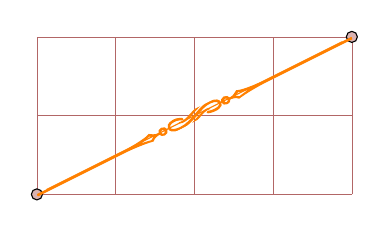
\begin{tikzpicture}
\node (A) at (0,0) {};
\node (B) at (4,2) {};
\draw [help lines,color=Maroon!60]  (0,0) grid (4,2);
\draw [fill=Maroon!30]  (A) circle (2pt) (B) circle (2pt);
\draw [orange] (A)  to [ornament=88]   (B);
\end{tikzpicture}
\end{tkzexample}

\begin{marginfigure}[-3cm]
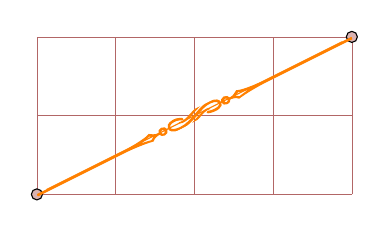
\begin{tikzpicture}
\node (A) at (0,0) {};
\node (B) at (4,2) {};
\draw [help lines,color=Maroon!60]  (0,0) grid (4,2);
\draw [fill=Maroon!30]  (A) circle (2pt) (B) circle (2pt);
\draw [orange] (A)  to [ornament=88]   (B);
\end{tikzpicture}
\caption{One ornament between two nodes}
\end{marginfigure}

\medskip
The next code shows how to place two ornaments between two nodes.

\begin{tkzexample}[code only,very small]
  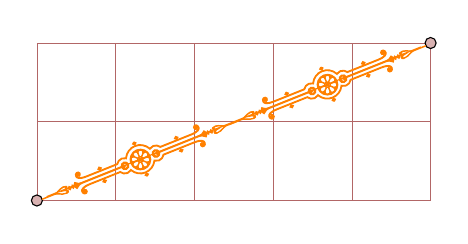
\begin{tikzpicture}
  \node (A) at (0,0) {};
  \node (B) at (5,2) {};
  \draw [help lines,color=Maroon!60]  (0,0) grid (5,2);
  \draw [fill=Maroon!30]  (A) circle (2pt) (B) circle (2pt);
  \path (A)--(B) coordinate[pos=.5] (c1);
  \draw [orange] (A)  to [ornament=84]
                 (c1) to [ornament=84] (B);
  \end{tikzpicture}
\end{tkzexample}


\begin{marginfigure}[-3cm]
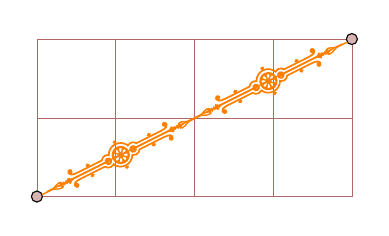
\begin{tikzpicture}
\node (A) at (0,0) {};
\node (B) at (4,2) {};
\draw [help lines,color=Maroon!60]  (0,0) grid (4,2);
\draw [fill=Maroon!30]  (A) circle (2pt) (B) circle (2pt);
\path (A)--(B) coordinate[pos=.5] (c1);
\draw [orange] (A)  to [ornament=84]
               (c1) to [ornament=84] (B);
\end{tikzpicture}
\caption{Two ornaments between two nodes}
\end{marginfigure}

\medskip
Example  with a pentagon

\begin{tkzexample}[code only,very small]
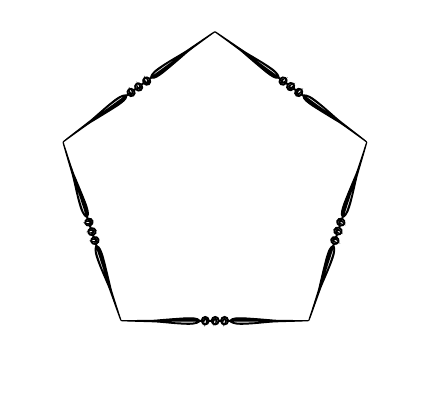
\begin{tikzpicture}[every node={anchor=center,
                                 inner sep=0pt}]
 \node[regular polygon, regular polygon sides=5,
 rotate=36,minimum size=5cm,inner sep=0pt](s)  {};
 \path (s.side 1) to [ornament=83] (s.side 2)
                  to [ornament=83] (s.side 3)
                  to [ornament=83] (s.side 4)
                  to [ornament=83] (s.side 5)
                  to [ornament=83] (s.side 1);
\end{tikzpicture}
\end{tkzexample}

\begin{marginfigure}
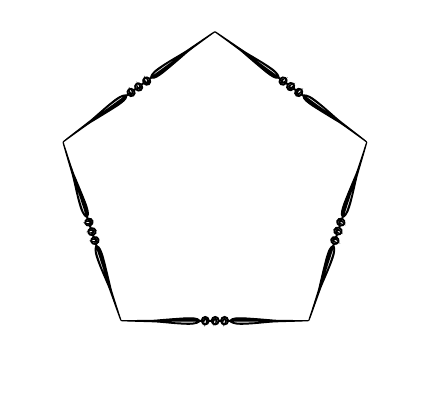
\begin{tikzpicture}[every node={anchor=center,
                                 inner sep=0pt}]
 \node[regular polygon, regular polygon sides=5,
 rotate=36,minimum size=5cm,inner sep=0pt](s)  {};
 \path (s.side 1) to [ornament=83] (s.side 2)
                  to [ornament=83] (s.side 3)
                  to [ornament=83] (s.side 4)
                  to [ornament=83] (s.side 5)
                  to [ornament=83] (s.side 1);
\end{tikzpicture}
\caption{A pentagon}
\end{marginfigure}

\subsection{How to use the option \tkzname{ornament/at}} \index{ornament/at}
\label{sub:how_to_use_the_option_at}

It's possible to move the ornament on the line AB. You only need to write \tkzname{at = number} where number is a percent like  \tkzname{pos}.
\begin{tkzexample}[code only,very small]
  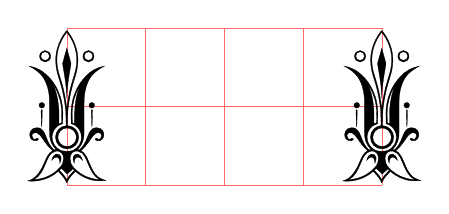
\begin{tikzpicture}
  \node (A) at (0,0) {};
  \node (B) at (4,0) {};
  \draw [help lines,color=red!60]  (0,-1) grid (4,1);
  \path  (A.center)  to [ornament=67,ornament/at=0,
                options/.append style={scale=.25}]   (B.center);
  \path  (A.center)  to [ornament=67,ornament/at=1,
                options/.append style={scale=.25}]   (B.center);
  \end{tikzpicture}
\end{tkzexample}

\begin{marginfigure}
  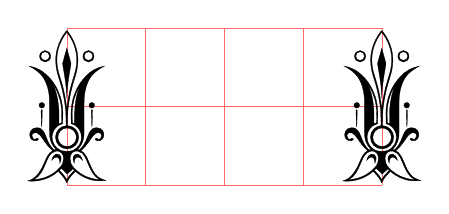
\begin{tikzpicture}
  \node (A) at (0,0) {};
  \node (B) at (4,0) {};
  \draw [help lines,color=red!60]  (0,-1) grid (4,1);
  \path  (A.center)  to [ornament=67,ornament/at=0,
                options/.append style={scale=.25}]   (B.center);
  \path  (A.center)  to [ornament=67,ornament/at=1,
                options/.append style={scale=.25}]   (B.center);
  \end{tikzpicture}
  \caption{option at}
\end{marginfigure}


\subsection{How to use the option \tkzname{options}}
\label{sub:how_to_use_the_option_options}

If an ornament is misplaced we can  move it up or down. Look at the code to see how to use \tkzname{options}.  \index{options}

\begin{tkzexample}[code only,very small]
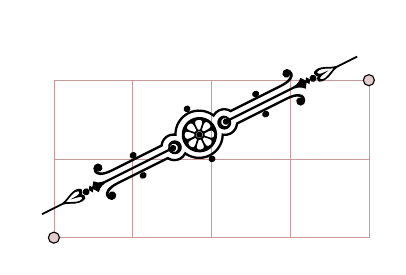
\begin{tikzpicture}
\node (A) at (0,0) {};
\node (B) at (4,2) {};
\draw [help lines,color=Maroon!40]  (0,0) grid (4,2);
\draw [fill=Maroon!20]  (A) circle (2pt) (B) circle (2pt);
\path  (A.center) to [ornament=84,
       options/.append style={yshift=10pt}] (B.center);
\end{tikzpicture}
\end{tkzexample}

\begin{marginfigure}[-3cm]
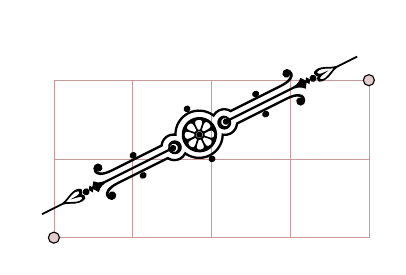
\begin{tikzpicture}
\node (A) at (0,0) {};
\node (B) at (4,2) {};
\draw [help lines,color=Maroon!40]  (0,0) grid (4,2);
\draw [fill=Maroon!20]  (A) circle (2pt) (B) circle (2pt);
\path  (A.center) to [ornament=84,
        options/.append style={yshift=10pt}] (B.center);
\end{tikzpicture}
\caption{How options}
\end{marginfigure}

\section{How to make a line of ornaments}
\subsection{With the chains library}
\begin{marginfigure}

\begin{tikzpicture}
  \node[draw,circle,minimum size=4pt,inner sep=0] (A) at (0,0){};
  \coordinate (B) at (8,0);
  {[start chain,node distance=0,inner sep=0]
  \node[anchor=west] [on chain] at (A){\pgfornament[width=1cm]{70}};
\node [on chain] {\pgfornament[width=1cm]{70}};
\node [on chain] {\pgfornament[width=1cm]{70}};
\node [on chain] {\pgfornament[width=1cm]{70}};}
  \end{tikzpicture}
  \caption{Line with \doclib{chains} library}
\end{marginfigure}

\begin{tkzexample}[code only,very small]

\begin{tikzpicture}
\node[draw,circle,
     minimum size=4pt,inner sep=0] (A) at (0,0){};
\coordinate (B) at (8,0);
{[start chain,node distance=0,inner sep=0]
\node[anchor=west] [on chain] at (A){\pgfornament[width=1cm]{70}};
\node [on chain] {\pgfornament[width=1cm]{70}};
\node [on chain] {\pgfornament[width=1cm]{70}};
\node [on chain] {\pgfornament[width=1cm]{70}};}
\end{tikzpicture}
\end{tkzexample}

\subsection{With the macro  \doccmd{pgfornamentline}}

Autopsy of this macro, you need 4 mandatory arguments: first of all two points between which the line is placed, the number of ornaments to create the line and of course the number of the ornament.
An optional argument allows you to set options.

\begin{marginfigure}
  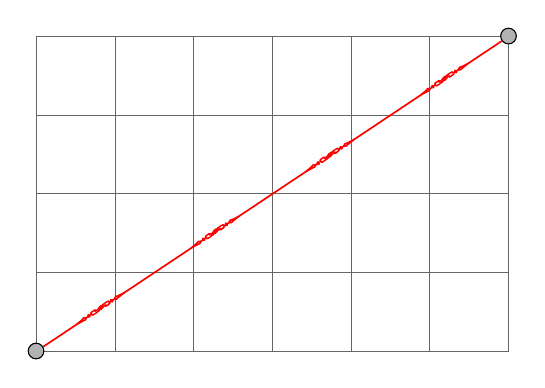
\begin{tikzpicture}[bullet/.style={circle,draw,fill=black!30,inner sep=2pt}]
  \draw [help lines,color=black!60]  (0,0) grid (6,4);
  \node[bullet] (A) at (0,0) {};
  \node[bullet] (B) at (6,4) {};
  \pgfornamentline[color=red]{A}{B}{4}{88}
  \end{tikzpicture}
  \caption{A line with ornaments}
\end{marginfigure}

\begin{tkzexample}[code only, very small]
  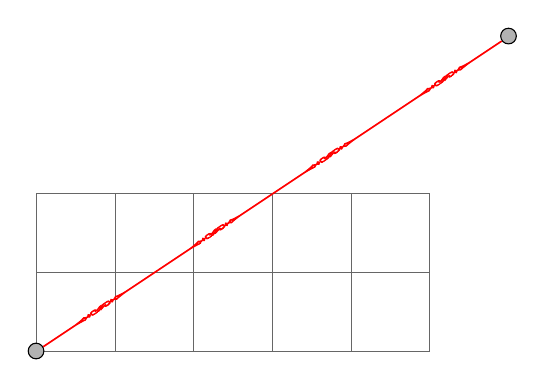
\begin{tikzpicture}[bullet/.style={%
            circle,draw,fill=black!30,inner sep=2pt}]
  \draw [help lines,color=black!60]  (0,0) grid (5,2);
  \node[bullet] (A) at (0,0) {};
  \node[bullet] (B) at (6,4) {};
  \pgfornamentline[color=red]{A}{B}{4}{88}
  \end{tikzpicture}
\end{tkzexample}



\section{Place ornaments with \doclib{chains} on a circle}
\begin{marginfigure}
  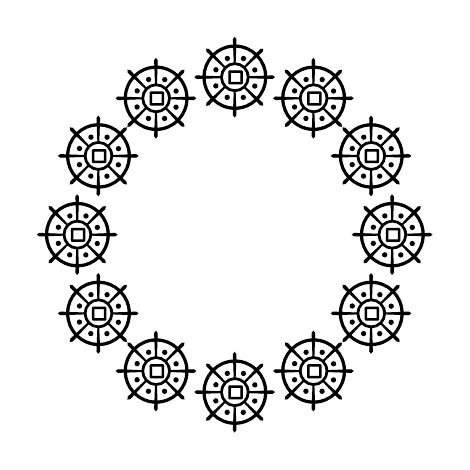
\begin{tikzpicture}[start chain=circle placed {at=(\tikzchaincount*30:2)}]
  \foreach \i in {1,...,12} \node [on chain] {\pgfornament[width=1cm]{4}};
  \end{tikzpicture}
  \caption{ A circle with ornaments}
\end{marginfigure}

\begin{tkzexample}[code only,very small]
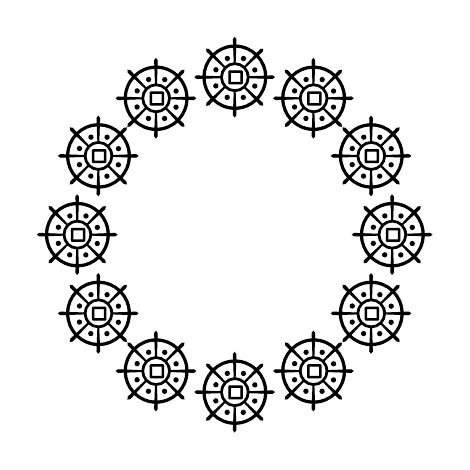
\begin{tikzpicture}[start chain=circle placed %
     {at=(\tikzchaincount*30:2)}]
\foreach \i in {1,...,12} \node [on chain]%
    {\pgfornament[width=1cm]{4}};
\end{tikzpicture}
\end{tkzexample}


\section{Vectorian Library} 
\label{sec:vectorian}
\subsection{Ornaments : Vector Symbols}
\label{sec:ornaments_symbols}
Here a list of the first thirty  elements
\subsection{Symbols part 1}
\label{sub:symbol1}
\index{ornament!symbols1a}
\ornamentview{1,...,30,97,98,140,141}%
\label{tab:ornaments : symbol1}

\subsection{Symbols part 2}
\label{sub:symbol2}
Tsubhe next  list is about symbols of decoration. The design is more sophisticated. Be careful indices range from sixty-five to seventy-nine.
\index{ornament!symbols2}%
\parindent=0pt

\medskip
\ornamentview{65,...,79}%
\label{tab:ornaments : symbol2}

\subsection{Ornaments : Vector Corners}
\label{sec:corners}
 The next list of ornaments concerns objects to place in the corners of a figure.  Half of them is not useful because it is obtained by symmetry of the other.

\index{ornament!corners1}
\ornamentview{31,...,42,61,62,63,64}%
\label{tab:ornaments : corners1}

\index{ornament!corners2}
\ornamentview{131,132,194,195}%
\label{tab:ornaments : corners2}

\subsection{Ornaments : Vector Lines}
\label{sec:lines}
The next list concerns symbols used to make a line.
\index{ornament!lines}

\medskip
\ornamentview{80,89}%
\label{tab:ornaments : lines}

\subsection{Ornaments : Animals}
\label{sec:animal }
The next list concerns symbols with animals.
\index{ornament!Animals}

\medskip
\ornamentview{90,91,100,102,104,106,107,108,109,110,111,112,113,122,123,124,158,159,133,134,135,136,156,157,158,159,190,193,137}%
\label{tab:ornaments : animal}

\subsection{Ornaments : Hands}
\label{sec:hands }
Remark : Ornaments 154 and 155 are identic but their sizes are smaller.

\medskip
\ornamentview{152,153,154,155}%
\label{tab:ornaments : hands}

\subsection{Ornaments : Humans}
\label{sec:humans}
 Remark : Ornaments 143, 144 and 145, 146 are identic but their sizes are different.

\medskip
\ornamentview{95,103,105,125,143,144,160,164}%
\label{tab:ornaments : humans}

\subsection{Ornaments : Objects}
\label{tab:ornaments : objects}

\medskip
\ornamentview{92,...,95,114,...,121,126,...,131,147,148,151,162,...,189,191,192}

\newpage
\section{Chinese traditional motifs}

This library of Chinese motifs is the work of two people: \emph{LianTze Lim} and \emph{Chennan Zhang}. They've been trying to provide some of the traditional patterns of the Han style using the existing mechanism of \texttt{pgfornament}. All patterns were finalized by \emph{Chennan Zhang} in CAD, drawn by TikZ, and converted by \emph{LianTze Lim} into macro package code suitable for the \texttt{pgfornament} mechanism. Thispackage is called \texttt{pgfornament-han}. Now I've incorporated the patterns directly... 
\ClearShipoutPictureBG
\newpgfornamentfamily{pgfhan}

\begingroup
\color{MidnightBlue}
\subsection{Corner symbols for connecting simple lines}
\label{sub:corner simple}
\ornamentview{1,...,8}%

\subsection{Corner symbols for connecting double lines}
\label{sub:corner double}
\ornamentview{9,...,14}%

\subsection{Corner symbols}
\label{sub:corner symbols}
\ornamentview{19,...,28}%

\subsection{Single line, double line, straight line}
\label{sub:corner symbols}
\ornamentview{29,...,32}%

\subsection{Other symbols}
\label{sub:other symbols}
\ornamentview{33,...,78}%
\endgroup


\newpgfornamentfamily{vectorian}


\subsection{Frame around a page}
Here the code to the frame auround the page
\begin{tkzexample}[code only,very small]
\AddToShipoutPicture{%
\begingroup
\setlength{\@tempdima}{2mm}%
\setlength{\@tempdimb}{\paperwidth-\@tempdima-1cm}%
\setlength{\@tempdimc}{\paperheight-\@tempdima}%
\put(\LenToUnit{\@tempdima},\LenToUnit{\@tempdimc}){%
  \pgfornament[color=Maroon,anchor=north west,width=1cm]{39}}
\put(\LenToUnit{\@tempdima},\LenToUnit{\@tempdima}){%
  \pgfornament[color=Maroon,anchor=south west,width=1cm,symmetry=h]{39}}
\put(\LenToUnit{\@tempdimb},\LenToUnit{\@tempdimc}){%
  \pgfornament[color=Maroon,anchor=north east,width=1cm,symmetry=v]{39}}
\put(\LenToUnit{\@tempdimb},\LenToUnit{\@tempdima}){%
  \pgfornament[color=Maroon,anchor=south east,width=1cm,symmetry=c]{39}}
\endgroup
}
\let\strippt\strip@pt
\end{tkzexample}

\clearpage\newpage
\section{Application: Placing corners}
\label{sec:application_placement}
Remark : Corners are the same dimensions ( width = height )

\begin{figure}[h!]
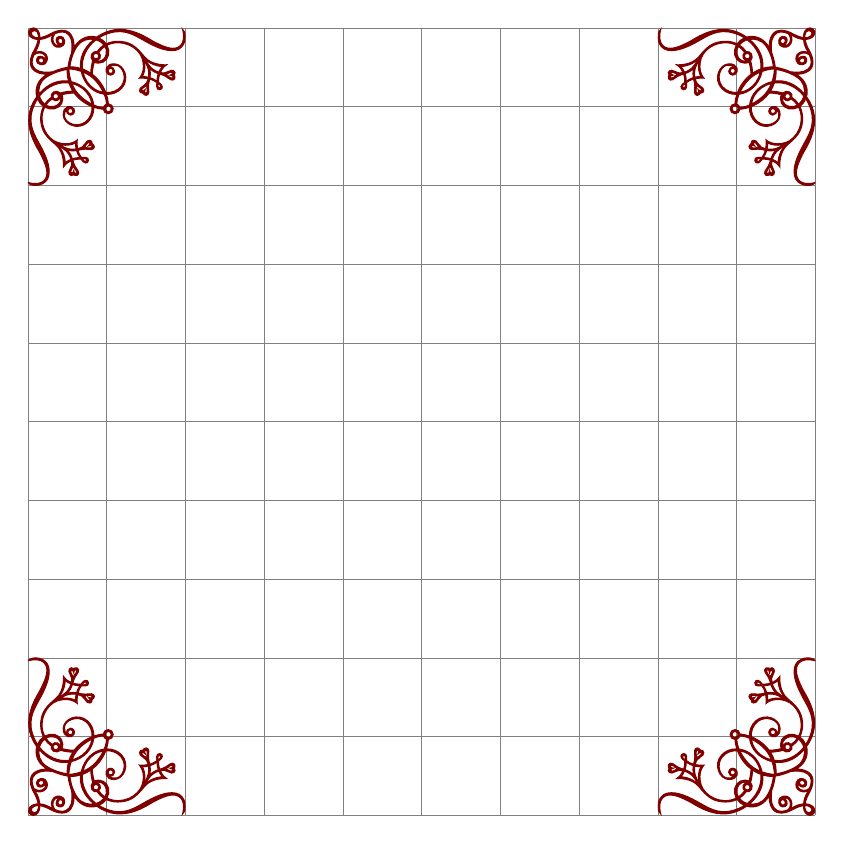
\begin{tikzpicture}[color=Maroon,every node/.style={inner sep=0pt}]
\draw[help lines] (-5,-5) grid (5,5);
\node[minimum size=10cm](vecbox){};
\node[anchor=north west] at (vecbox.north west){\pgfornament[width=2cm]{61}};
\node[anchor=north east] at (vecbox.north east){\pgfornament[width=2cm,symmetry=v]{61}};
\node[anchor=south west] at (vecbox.south west){\pgfornament[width=2cm,symmetry=h]{61}};
\node[anchor=south east] at (vecbox.south east){\pgfornament[width=2cm,symmetry=c]{61}};
\end{tikzpicture}
\caption{Placing corners}
\end{figure}


\begin{tkzexample}[code only,very small]
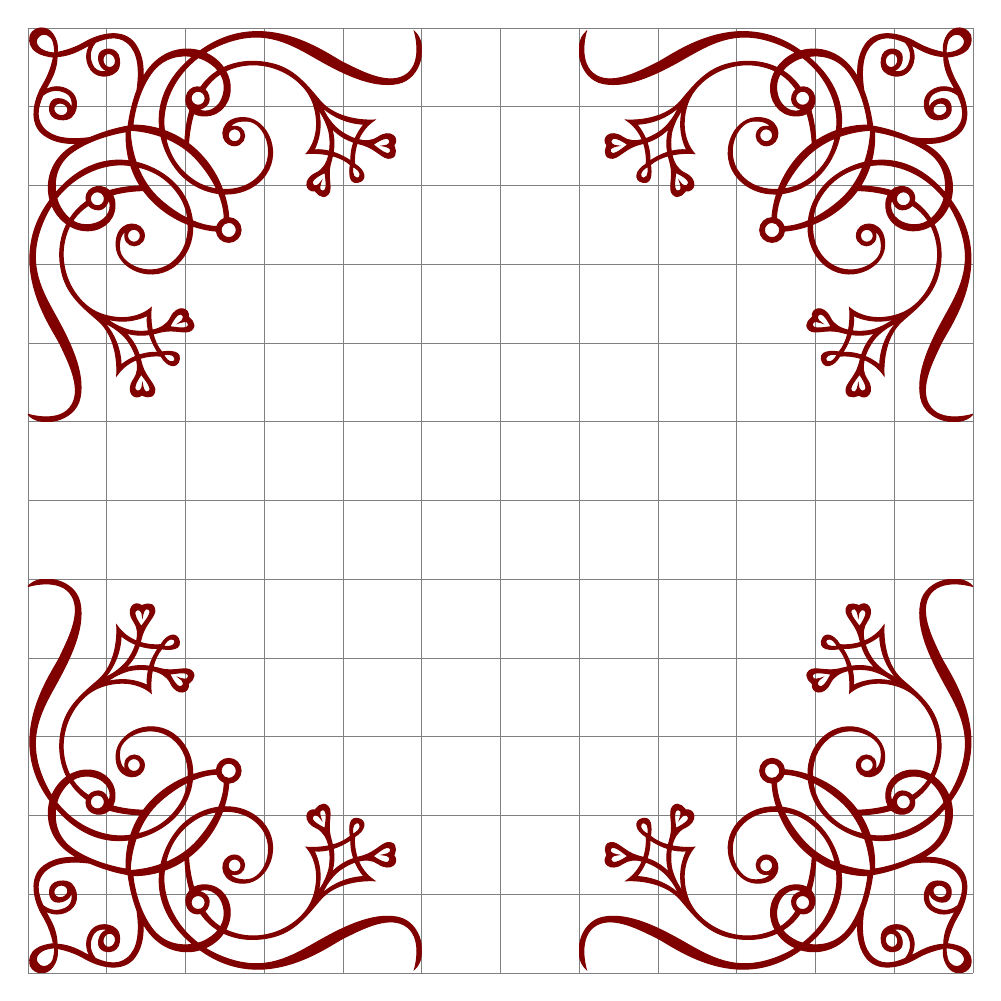
\begin{tikzpicture}[color=Maroon,
                    every node/.style={inner sep=0pt}]
 \draw[help lines] (-6,-6) grid (6,6);
 \node[minimum size=12cm](vecbox){};
 \node[anchor=north west] at (vecbox.north west)
      {\pgfornament[width=5cm]{61}};
 \node[anchor=north east] at (vecbox.north east)
      {\pgfornament[width=5cm,symmetry=v]{61}};
 \node[anchor=south west] at (vecbox.south west)
      {\pgfornament[width=5cm,symmetry=h]{61}};
 \node[anchor=south east] at (vecbox.south east)
      {\pgfornament[width=5cm,symmetry=c]{61}};
\end{tikzpicture}
\end{tkzexample}
\index{minimum size}
\index{anchor}

\section{Application: Create a frame for the page}

\begin{tikzpicture}[remember picture, overlay]
\node[anchor=north west] (nw) at (current page.north west){%
\pgfornament[width=2cm]{63}};
\node[anchor=north east] (ne) at (current page.north east){%
\pgfornament[width=2cm,symmetry=v]{63}};
\node[anchor=south west] (sw) at (current page.south west){%
\pgfornament[width=2cm,symmetry=h]{63}};
\node[anchor=south east] (se) at (current page.south east){%
\pgfornament[width=2cm,symmetry=c]{63}};
\coordinate (nw) at ([shift={(-.82cm,-1cm)}]nw);
\coordinate (sw) at ([shift={(-.82cm,+1cm)}]sw);
\coordinate (ne) at ([shift={(+.82cm,-1cm)}]ne);
\coordinate (se) at ([shift={(+.82cm,+1cm)}]se);
\pgfornamentline[color=Maroon]{nw}{sw}{4}{88}
\pgfornamentline[color=Maroon]{ne}{se}{4}{88}
\coordinate (nw) at ([shift={(1.8 cm,1.845 cm)}]nw);
\coordinate (ne) at ([shift={(-1.8 cm,1.845 cm)}]ne);
\pgfornamentline[color=Maroon]{nw}{ne}{3}{88}
\coordinate (sw) at ([shift={(1.8 cm,-1.845 cm)}]sw);
\coordinate (se) at ([shift={(-1.8 cm,-1.845 cm)}]se);
\pgfornamentline[color=Maroon]{sw}{se}{3}{88}
\pgfornamentline[color=Maroon]{sw}{se}{3}{88}
\end{tikzpicture}


\section{Application: Frame around a text}
\label{sec:application_poem}
I chose a poem to illustrate this theme.


\begin{center}
\begin{figure}[h!]
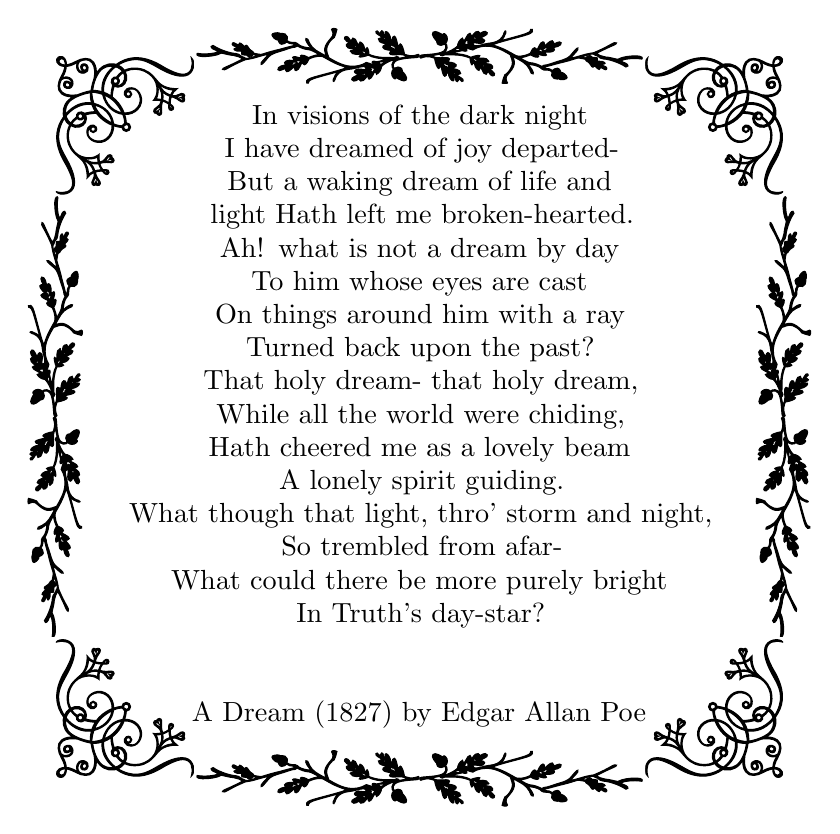
\begin{tikzpicture}
  \node[text width=8cm,align=center](Text){%
  In visions of the dark night\\
  I have dreamed of joy departed-\\
  But a waking dream of life and light\
  Hath left me broken-hearted.\\

  Ah! what is not a dream by day\\
  To him whose eyes are cast \\
  On things around him with a ray \\
  Turned back upon the past? \\

  That holy dream- that holy dream,\\
  While all the world were chiding,\\
  Hath cheered me as a lovely beam\\
  A lonely spirit guiding.\\

  What though that light, thro' storm and night,\\
  So trembled from afar- \\
  What could there be more purely bright \\
  In Truth's day-star? \\
  \vspace{24pt}
   A Dream (1827) by Edgar Allan Poe
  } ;

\node[inner sep=0pt,shift={(-.5cm,.5cm)},anchor=north west](CNW)  at (Text.north west)
    {\pgfornament[width=1.75cm]{61}};
\node[inner sep=0pt,shift={(.5cm,.5cm)},anchor=north east](CNE)   at (Text.north east)
    {\pgfornament[width=1.75cm,symmetry=v]{61}};
\node[inner sep=0pt,shift={(-.5cm,-.5cm)},anchor=south west](CSW) at (Text.south west)
     {\pgfornament[width=1.75cm,symmetry=h]{61}};
\node[inner sep=0pt,shift={(.5cm,-.5cm)},anchor=south east](CSE)  at (Text.south east)
     {\pgfornament[width=1.75cm,symmetry=c]{61}};
 \pgfornamenthline{CNW}{CNE}{north}{87}
\pgfornamenthline{CSW}{CSE}{south}{87}
\pgfornamentvline{CNW}{CSW}{west}{87}
\pgfornamentvline{CNE}{CSE}{east}{87}
\end{tikzpicture}
\caption{A poem}
\end{figure}
\end{center}

The poem is placed in a node named \Verb+Text+.
Then we can place the corners relatively to four anchors of the node \Verb+Text+.
Finally with the macros \doccmd{pgfornamenthline}  and  \doccmd{pgfornamentvline} it's possible to finish the frame.

\begin{tkzexample}[code only,very small]

\begin{tikzpicture}[every node/.style={inner sep=0pt}]
\node[text width=8cm,align=center](Text){%
    In visions of the dark night ...} ;
\node[shift={(-1cm,1cm)},anchor=north west](CNW)
at (Text.north west) {\pgfornament[width=1.75cm]{61}};
\node[shift={(1cm,1cm)},anchor=north east](CNE)
at (Text.north east) {\pgfornament[width=1.75cm,symmetry=v]{61}};
\node[shift={(-1cm,-1cm)},anchor=south west](CSW)
at (Text.south west) {\pgfornament[width=1.75cm,symmetry=h]{61}};
\node[shift={(1cm,-1cm)},anchor=south east](CSE)
at (Text.south east) {\pgfornament[width=1.75cm,symmetry=c]{61}};
\pgfornamenthline{CNW}{CNE}{north}{87}
\pgfornamenthline{CSW}{CSE}{south}{87}
\pgfornamentvline{CNW}{CSW}{west}{87}
\pgfornamentvline{CNE}{CSE}{east}{87}
\end{tikzpicture}
\end{tkzexample}

\section{Application: Text inside a frame}
\label{sec:frame}
Firstly we build the frame with the help of nodes and the we place the text in a node relatively to others nodes.

\begin{figure}[h!]
\begin{center}
\newcommand{\framesize}{8 cm}
\begin{tikzpicture}[color=Maroon,
                   transform shape,
                   every node/.style={inner sep=0pt}]
\node[minimum size=\framesize,fill=Beige!20](vecbox){};
\node[anchor=north west] at (vecbox.north west){%
      \pgfornament[width=0.2*\framesize]{63}};
\node[anchor=north east] at (vecbox.north east){%
                         \pgfornament[width=0.2*\framesize,symmetry=v]{63}};
\node[anchor=south west] at (vecbox.south west){%
      \pgfornament[width=0.2*\framesize,symmetry=h]{63}};
\node[anchor=south east] at (vecbox.south east){%
      \pgfornament[width=0.2*\framesize,symmetry=c]{63}};
\node[anchor=north] at (vecbox.north){%
      \pgfornament[width=0.6*\framesize,symmetry=h]{46}};
\node[anchor=south] at (vecbox.south){%
      \pgfornament[width=0.6*\framesize]{46}};
\node[anchor=north,rotate=90]  at (vecbox.west){%
      \pgfornament[width=0.6*\framesize,symmetry=h]{46}};
\node[anchor=north,rotate=-90] at (vecbox.east){%
      \pgfornament[width=0.6*\framesize,symmetry=h]{46}};
\node[inner sep=6pt] (text) at (vecbox.center){\Huge Ornaments};
\node[anchor=north] at (text.south){%
      \pgfornament[width=0.5*\framesize]{75}};
\node[anchor=south] at (text.north){%
      \pgfornament[width=0.5*\framesize,symmetry=h]{75}};
\end{tikzpicture}
\caption{Text inside a frame with a tikzpicture's environment}
\end{center}
\end{figure}

\begin{tkzexample}[code only,very small]
\newcommand{\framesize}{8 cm}
\begin{tikzpicture}[color=Maroon,
                   transform shape,
                   every node/.style={inner sep=0pt}]
\node[minimum size=\framesize,fill=Beige!10](vecbox){};
\node[anchor=north west] at (vecbox.north west){%
      \pgfornament[width=0.2*\framesize]{63}};
\node[anchor=north east] at (vecbox.north east){%
      \pgfornament[width=0.2*\framesize,symmetry=v]{63}};
\node[anchor=south west] at (vecbox.south west){%
      \pgfornament[width=0.2*\framesize,symmetry=h]{63}};
\node[anchor=south east] at (vecbox.south east){%
      \pgfornament[width=0.2*\framesize,symmetry=c]{63}};
\node[anchor=north] at (vecbox.north){%
      \pgfornament[width=0.6*\framesize,symmetry=h]{46}};
\node[anchor=south] at (vecbox.south){%
      \pgfornament[width=0.6*\framesize]{46}};
\node[anchor=north,rotate=90]  at (vecbox.west){%
      \pgfornament[width=0.6*\framesize,symmetry=h]{46}};
\node[anchor=north,rotate=-90] at (vecbox.east){%
      \pgfornament[width=0.6*\framesize,symmetry=h]{46}};
\node[inner sep=6pt] (text) at (vecbox.center){\Huge Ornaments};
\node[anchor=north] at (text.south){%
      \pgfornament[width=0.5*\framesize]{75}};
\node[anchor=south] at (text.north){%
      \pgfornament[width=0.5*\framesize,symmetry=h]{75}};
\end{tikzpicture}
\end{tkzexample}
\index{transform shape}
\index{color}
\index{every node}

\section{Application: Other way to get a pentagon}
\label{sec:application_other_way_to_get_a_pentagon}
We can place ornaments manually but the last method can also be used .
\sidenote{\tkzcname{getornamentlength} is ...}

\begin{tkzexample}[code only,very small]
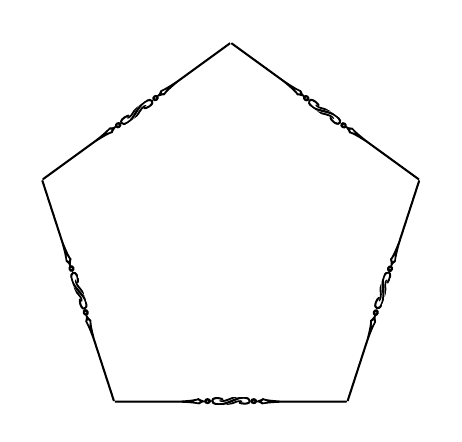
\begin{tikzpicture}[every node={anchor=center,inner sep=0pt}]
    \node[regular polygon,
          regular polygon sides=5,
          minimum size=5cm,
          inner sep=0pt](s)  {};
    \getornamentlength{s}{corner 1}{s}{corner 2}
    \node[rotate=216] at (s.side 1)
         {\pgfornament[width=\ornamentlen]{88}};
    \node[rotate=288] at (s.side 2)
         {\pgfornament[width=\ornamentlen]{88}};
    \node[rotate=0]   at (s.side 3)
         {\pgfornament[width=\ornamentlen]{88}};
    \node[rotate=72]  at (s.side 4)
         {\pgfornament[width=\ornamentlen]{88}};
    \node[rotate=144] at (s.side 5)
         {\pgfornament[width=\ornamentlen]{88}};
\end{tikzpicture}
\end{tkzexample}  \index{rotate}   \index{regular polygon}


\begin{marginfigure}[-1cm]
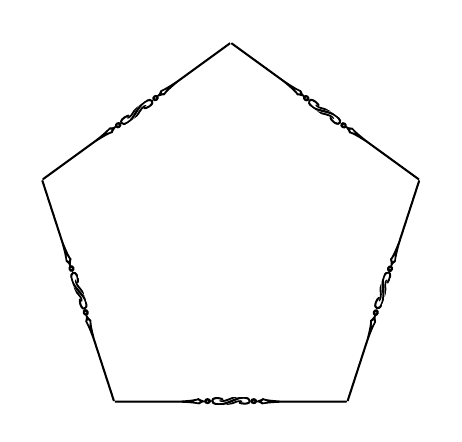
\begin{tikzpicture}[every node={anchor=center,inner sep=0pt}]
\node[regular polygon, regular polygon sides=5, 
      minimum size=5cm,inner sep=0pt](s)  {};
\getornamentlength{s}{corner 1}{s}{corner 2}
\node[rotate=216] at (s.side 1){\pgfornament[width=\ornamentlen]{88}};
\node[rotate=288] at (s.side 2){\pgfornament[width=\ornamentlen]{88}};
\node[rotate=0]   at (s.side 3){\pgfornament[width=\ornamentlen]{88}};
\node[rotate=72]  at (s.side 4){\pgfornament[width=\ornamentlen]{88}};
\node[rotate=144] at (s.side 5){\pgfornament[width=\ornamentlen]{88}};
\end{tikzpicture}
\caption{A pentagon}
\end{marginfigure}

\vspace{60pt}
\section{Package \docpkg{tikzrput}}
\label{sec:package_rput}

Pstricks Users are accustomed to placing objects with \doccmd{rput}\index{rput}, so I created a package \tkzname{\docpkg{tikzrput}} with only one macro \tkzcname{rput}. This macro is used as that of Pstricks with the same argument and options. Next to the document you are reading, you will find documentation on this package. The display of an object at the point $(x,y)$ is realized with \verb|\rput| of \emph{pstricks} like this :\par\medskip

\begin{docspec}
 \color{black} \doccmd{rput}[\docopt{refpoint}]\{\docarg{angle}\}%
\docparen{x,y}\{\doccmd{pgfornament[\docopt{options}]\{\docarg{number}\}}\}
\end{docspec}

\subsection{Example with \tkzcname{rput}}
\label{sub:example_with_rput}

\begin{tkzexample}[code only,very small]
\foreach \a in {0,4,...,356}{%
  \rput(\a;2){$\bullet$}%
  }
    \rput[B](0;0){Circle}%
\end{tkzexample}  \Imacro{foreach}

\begin{marginfigure}[-3cm]
\hspace*{2cm}
  \foreach \a in {0,16,...,356}{%
    \rput(\a;2){$\bullet$}%
    }
      \rput[B](0;0){Circle}%

  \vspace*{3cm}
      \caption{Example with \tkzcname{rput}}
\end{marginfigure}

\subsection{Ornament with  \tkzcname{rput}}
\label{sub:ornament_with}

\setlength{\fboxsep}{0pt}

\begin{tkzexample}[code only,very small]
\begin{picture}(5,4)
 \rput(2,1){\pgfornament[width=2cm]{1}}
 \rput(4,2){\pgfornament[width=2cm]{2}}
\end{picture}
\end{tkzexample} \Imacro{rput}

\begin{marginfigure}
  \begin{picture}(5,4)
   \rput(2,1){\pgfornament[color=CadetBlue,width=2cm]{1}}
   \rput(4,2){\pgfornament[color=CadetBlue,width=2cm]{2}}
  \end{picture}
 \caption{Placement with  rput}
\end{marginfigure}

\section{Examples from pgfornamenthan}
\label{sec:pgfornamenthan}
\ClearShipoutPictureBG
\newpgfornamentfamily{pgfhan}

\subsection{Example 1 from LianTze Lim}
\label{sub:LianTze1}
\url{https://github.com/liantze/pgfornament-han}

\begin{marginfigure}
\begin{center}

\begin{tikzpicture}
\tikzset{every node/.append style={inner sep=0pt,color=MidnightBlue!50}}
\tikzset{pgfornamentstyle/.style={draw=green!20!black,
           fill=orange,fill opacity=.5,thick}}%
\node (nw) {\pgfornament[scale=0.25]{12}};
\node[right=50bp of nw] (ne) {\pgfornament[scale=0.25,symmetry=v]{12}};
\node[below=50bp of nw] (sw) {\pgfornament[scale=0.25,symmetry=h]{12}};
\node[below=50bp of ne] (se) {\pgfornament[scale=0.25,symmetry=c]{12}};
\node[anchor=north west] at (nw.north east) {\pgfornament[scale=0.25]{32}};
\node[anchor=south west] at (sw.south east) {\pgfornament[scale=0.25]{32}};
\node[anchor=south west,rotate=-90] at (nw.south west)
                                  {\pgfornament[scale=0.25]{32}};
\node[anchor=south east,rotate=90] at (ne.south east)
                                  {\pgfornament[scale=0.25]{32}};

\node[anchor=center,shift={(25bp,-25bp)}] at (nw.south east) {\pgfornament[scale=0.5]{57}};
\end{tikzpicture}
\caption{Example 1 LianTze Lim }
\end{center}
\end{marginfigure}
\begin{tkzexample}[code only,very small]

\begin{tikzpicture}
\tikzset{every node/.append style={inner sep=0pt,color=MidnightBlue!50}}
\tikzset{pgfornamentstyle/.style={draw=green!20!black,
           fill=orange,fill opacity=.5,thick}}%
\node (nw) {\pgfornament[scale=0.25]{12}};
\node[right=50bp of nw] (ne){\pgfornament[scale=0.25,symmetry=v]{12}};
\node[below=50bp of nw] (sw){\pgfornament[scale=0.25,symmetry=h]{12}};
\node[below=50bp of ne] (se){\pgfornament[scale=0.25,symmetry=c]{12}};
\node[anchor=north west] at (nw.north east)%
             {\pgfornament[scale=0.25]{32}};
\node[anchor=south west] at (sw.south east)%
             {\pgfornament[scale=0.25]{32}};
\node[anchor=south west,rotate=-90] at (nw.south west)
                            {\pgfornament[scale=0.25]{32}};
\node[anchor=south east,rotate=90] at (ne.south east)
                            {\pgfornament[scale=0.25]{32}};
\node[anchor=center,shift={(25bp,-25bp)}] at (nw.south east)
 {\pgfornament[scale=0.5]{57}};
\end{tikzpicture}
\end{tkzexample}

\subsection{Example 2 from LianTze Lim}


\begin{marginfigure}
\begin{center}

\begin{tikzpicture}
\tikzset{every node/.append style={color=Goldenrod,inner sep=0pt}}
\node (nw) {\pgfornament[scale=0.25]{23}};
\node[right=53bp of nw] (ne) 
     {\pgfornament[scale=0.25,symmetry=v]{23}}; 
\node[anchor=north west,xshift=-2bp] at (nw.north east)   
     {\pgfornament[scale=0.25]{41}}; 
\node[anchor=north east,xshift=2bp] at (ne.north west)
     {\pgfornament[scale=0.25,symmetry=v]{41}}; 
\end{tikzpicture}
\end{center}
\caption{Example 2 LianTze Lim }
\end{marginfigure}
\begin{tkzexample}[code only,very small]

\begin{tikzpicture}
\tikzset{every node/.append style={color=Goldenrod,inner sep=0pt}}
\node (nw) {\pgfornament[scale=0.25]{23}};
\node[right=53bp of nw] (ne){\pgfornament[scale=0.4,symmetry=v]{23}};
 \node[anchor=north west,xshift=8bp] at (nw.north east)   
  {\pgfornament[scale=0.25]{41}}; 
\node[anchor=north east,xshift=-8bp] at (ne.north west)
  {\pgfornament[scale=0.25,symmetry=v]{41}}; 
\end{tikzpicture}
\end{tkzexample}


\clearpage\newpage
\subsection{Example 3 (based on an example of  LianTze Lim)}
\newpgfornamentfamily{pgfhan}

\newbox{\fortyseven}
\savebox{\fortyseven}{\pgfornament[scale=0.20,color=MidnightBlue]{47}}
\tikzset{every node/.append style={inner sep=0pt}}
\AddToShipoutPictureBG{\begin{tikzpicture}[overlay,remember picture,color=MidnightBlue]
\node[anchor=north west,shift={(0.7,-0.85)}] at (current page.north west)
  (nw) {\pgfornament[scale=0.2]{25}};
\node[anchor=north east,shift={(-0.7,-0.85)}] at (current page.north east)
  (ne) {\pgfornament[scale=0.2,symmetry=v]{25}};
\node[anchor=south west,shift={(0.7,0.85)}] at (current page.south west)
  (sw) {\pgfornament[scale=0.2,symmetry=h]{25}};
\node[anchor=south east,shift={(-0.7,0.85)}] at (current page.south east)
  (se) {\pgfornament[scale=0.2,symmetry=c]{25}};
\begin{scope}[start chain,node distance=-3pt]
\node[anchor=north west,on chain] at (nw.north east) {\usebox{\fortyseven}};
\foreach \i in {1,...,14} {\node[on chain]{\usebox{\fortyseven}};}
\end{scope}
 \begin{scope}[start chain,node distance=-3pt]
 \node[anchor=south west,on chain] at (sw.south east) {\usebox{\fortyseven}};
 \foreach \i in {1,...,6} \node[on chain]{\usebox{\fortyseven}};
 \end{scope}
\begin{scope}[start chain=going left,node distance=-3pt]
\node[anchor=south east,on chain,xshift={3pt}] at (se.south west) {\usebox{\fortyseven}};
\foreach \i in {1,...,6} \node[on chain]{\usebox{\fortyseven}};
\end{scope}
\foreach \i in {0,...,22}
  \node[anchor=south west,rotate=-90,shift={($\i*(31bp,0)$)}] at (nw.south west)
    {\usebox{\fortyseven}};
\foreach \i in {0,...,22}
  \node[anchor=south east,rotate=90,shift={($\i*(-31bp,0)$)}] at ([yshift={+3pt}]ne.south east)
    {\usebox{\fortyseven}};
\node[yshift=32pt] at (current page.south) {\pgfornament[scale=0.1]{51}};
\node[yshift=32pt,text=black] at (current page.south) {\large\thepage};
\end{tikzpicture}}

\begin{center}

\begin{tikzpicture}
  \tikzset{every node/.append style={MidnightBlue,inner sep=0pt,node distance=0pt}}
  \node (nw) {\pgfornament[scale=0.2]{6}};
  \node[right=100bp of nw] (ne){\pgfornament[scale=0.2,symmetry=v]{16}};
  \node[below=-8bp of nw] (sw) {\pgfornament[scale=0.2,symmetry=h]{16}};
  \node[below=-8bp of ne] (se) {\pgfornament[scale=0.2,symmetry=c]{6}};
  \node[anchor=north west,xscale=2.5] at (nw.north east)   
       {\pgfornament[scale=0.2]{30}};
  \node[anchor=south west,xscale=2.5] at (sw.south east) 
       {\pgfornament[scale=0.2]{30}};
  \node[font=\Large,text=black,shift={(50bp,4bp)}] at (nw.south east) {Code from the frame};
\end{tikzpicture}
\end{center}

\begin{tkzexample}[code only, very small]
\newpgfornamentfamily{pgfhan}
\newbox{\fortyseven}
\savebox{\fortyseven}{\pgfornament[scale=0.20,color=MidnightBlue]{47}}
\tikzset{every node/.append style={inner sep=0pt}}
\AddToShipoutPictureBG{%
\begin{tikzpicture}[overlay,remember picture,color=MidnightBlue]
\node[anchor=north west,shift={(0.7,-0.85)}] at (current page.north west)
  (nw) {\pgfornament[scale=0.2]{25}};
\node[anchor=north east,shift={(-0.7,-0.85)}] at (current page.north east)
  (ne) {\pgfornament[scale=0.2,symmetry=v]{25}};
\node[anchor=south west,shift={(0.7,0.85)}] at (current page.south west)
  (sw) {\pgfornament[scale=0.2,symmetry=h]{25}};
\node[anchor=south east,shift={(-0.7,0.85)}] at (current page.south east)
  (se) {\pgfornament[scale=0.2,symmetry=c]{25}};
\begin{scope}[start chain,node distance=-3pt]
\node[anchor=north west,on chain] at (nw.north east)
{\usebox{\fortyseven}};
\foreach \i in {1,...,14} {\node[on chain]{\usebox{\fortyseven}};}
\end{scope}
 \begin{scope}[start chain,node distance=-3pt]
 \node[anchor=south west,on chain] at (sw.south east)
 {\usebox{\fortyseven}};
 \foreach \i in {1,...,6} \node[on chain]{\usebox{\fortyseven}};
 \end{scope}
\begin{scope}[start chain=going left,node distance=-3pt]
\node[anchor=south east,on chain,xshift={3pt}] at (se.south west)
 {\usebox{\fortyseven}};
\foreach \i in {1,...,6} \node[on chain]
{\usebox{\fortyseven}};
\end{scope}
\foreach \i in {0,...,22}
\node[anchor=south west,rotate=-90,
      shift={($\i*(31bp,0)$)}] at (nw.south west)
      {\usebox{\fortyseven}};
\foreach \i in {0,...,22}
\node[anchor=south east,rotate=90,shift={($\i*(-31bp,0)$)}] at
 ([yshift={+3pt}]ne.south east){\usebox{\fortyseven}};
\node[yshift=32pt] at (current page.south){\pgfornament[scale=0.1]{51}};
\node[yshift=32pt,text=black] at (current page.south){\large\thepage};
\end{tikzpicture}
}
\end{tkzexample}

\clearpage \newpage
\subsection{Example 4 (based on an example of  LianTze Lim)}
\begin{figure}
\begin{newfamily}[pgfhan]
\begin{center}
  \begin{tikzpicture}
  \tikzset{every node/.append style={inner sep=0pt,color= MidnightBlue}} 
  \node[minimum width=180bp,minimum height=100bp] (chframe){};
  \node[anchor=north west] (nw) at (chframe.north west) 
    {\pgfornament[scale=0.25]{1}};
  \node[anchor=north east]  at (chframe.north east)    
    {\pgfornament[symmetry=v,scale=0.25]{1}};
  \node[anchor=south west] (sw) at (chframe.south west) 
    {\pgfornament[symmetry=h,scale=0.25]{1}};
  \node[anchor=south east]  at (chframe.south east) 
    {\pgfornament[symmetry=c,scale=0.25]{1}};
   \node[anchor=south west,xscale=2] at (sw.south east) 
    {\pgfornament[scale=0.25]{29}};
    \node[anchor=north west,xscale=2] at (nw.north east) 
    {\pgfornament[scale=0.25]{29}};
  % circle
  \begin{scope}
  \tikzset{pgfornamentstyle/.style={draw=Goldenrod,fill=Red,line width=1pt}}
  \node[fill=MidnightBlue,circle,draw=Red,line width=2pt,inner sep=-8pt]
  at (chframe.center)  {\pgfornament[scale=0.40]{56}};
  \end{scope}
  \end{tikzpicture}
\end{center}
\end{newfamily}
\end{figure}

\begin{tkzexample}[code only, very small]
\begin{newfamily}[pgfhan]
\begin{center}
\begin{tikzpicture}
\tikzset{every node/.append style={%
        inner sep=0pt,
        color= MidnightBlue}} 
\node[minimum width=180bp,minimum height=100bp] (chframe){};
\node[anchor=north west] (nw) at (chframe.north west) 
  {\pgfornament[scale=0.25]{1}};
\node[anchor=north east]  at (chframe.north east)    
  {\pgfornament[symmetry=v,scale=0.25]{1}};
\node[anchor=south west] (sw) at (chframe.south west) 
  {\pgfornament[symmetry=h,scale=0.25]{1}};
\node[anchor=south east]  at (chframe.south east) 
  {\pgfornament[symmetry=c,scale=0.25]{1}};
 \node[anchor=south west,xscale=2] at (sw.south east) 
  {\pgfornament[scale=0.25]{29}};
  \node[anchor=north west,xscale=2] at (nw.north east) 
  {\pgfornament[scale=0.25]{29}};
% circle
\begin{scope}
\tikzset{pgfornamentstyle/.style={draw=Goldenrod,
                                    fill=Red,
                                    line width=1pt}}
\node[fill=MidnightBlue,circle,draw=Red,
        line width=2pt,inner sep=-8pt]
  at (chframe.center) {\pgfornament[scale=0.40]{56}};
\end{scope}
\end{tikzpicture}
\end{center}
\end{newfamily}
\end{tkzexample}

\clearpage \newpage
\ClearShipoutPicture
\newpgfornamentfamily{vectorian}
\section{Examples from psvectorian}
\label{sec:psvectorian}

\subsection{Large Title -- e01}
\label{sub:largetitle}
This example is given  here :
\url{http://melusine.eu.org/syracuse/pstricks/vectorian/e01.tex}.

I use the macro \Verb|rput| from my package tikzrput to get the figure with the same code.
I only replace \doccmd{psvectorian} by \doccmd{pgfornament}.

\begin{figure}
  \begin{center}
  \rput[r](-3pt,3pt){\pgfornament[scale=.35]{72}}
  \Large{Motifs d'ornements}%
  \rput[l](3pt,3pt){\pgfornament[scale=.35]{73}}\\
  \rput(0,0){\pgfornament[scale=.5]{85}}
  \end{center}
  \caption{Example named e01 in psvectorian}
\end{figure}
\begin{tkzexample}[code only,very small]
  \rput[r](-3pt,3pt){\pgfornament[scale=.35]{72}}
  \large{Motifs d'ornements}%
  \rput[l](3pt,3pt){\pgfornament[scale=.35]{73}}\\
  \rput(0,0){\pgfornament[scale=.5]{85}}
\end{tkzexample}

\subsection{Cover with frame -- e02}
This example is given  here

{\small\url{http://melusine.eu.org/syracuse/pstricks/vectorian/e02.tex}}

I need  \docenv{tikzpicture} and \doccmd{draw} to replace \docenv{pspicture} and \doccmd{psframe}.

\begin{figure}
\begin{center}
  \begin{tikzpicture}[color=blue]
   \draw[use as bounding box,thin] (-5,-5) rectangle (5,5);
   \node {\rput[tl](-3,5){\pgfornament[width=6cm]{71}}
   \rput[bl](-3,-5){\pgfornament[width=6cm,,symmetry=h]{71}}
   \rput[tl](-5,5){\pgfornament[width=2cm]{63}}
   \rput[tr](5,5){\pgfornament[width=2cm,,symmetry=v]{63}}
   \rput[bl](-5,-5){\pgfornament[width=2cm,,symmetry=h]{63}}
   \rput[br](5,-5){\pgfornament[width=2cm,,symmetry=c]{63}}
   \rput[bl]{-90}(-5,3){\pgfornament[width=6cm]{46}}
   \rput[bl]{90}(5,-3){\pgfornament[width=6cm]{46}}
   \rput(0,0){\Huge Ornaments}
   \rput[t](0,-0.5){\pgfornament[width=5cm]{75}}
   \rput[b](0,0.5){\pgfornament[width=5cm]{69}}
   \rput[tr]{-30}(-1,2.5){\pgfornament[width=2cm]{57}}
   \rput[tl]{30}(1,2.5){\pgfornament[width=2cm,symmetry=v]{57}}};
   \end{tikzpicture}
\end{center}
\caption{Example named e02 in psvectorian}
\end{figure}

\begin{tkzexample}[code only,very small]
 \begin{tikzpicture}[color=blue]
  \draw[use as bounding box,thin] (-5,-5) rectangle (5,5);
  \node {\rput[tl](-3,5){\pgfornament[width=6cm]{71}}
  \rput[bl](-3,-5){\pgfornament[width=6cm,,symmetry=h]{71}}
  \rput[tl](-5,5){\pgfornament[width=2cm]{63}}
  \rput[tr](5,5){\pgfornament[width=2cm,,symmetry=v]{63}}
  \rput[bl](-5,-5){\pgfornament[width=2cm,,symmetry=h]{63}}
  \rput[br](5,-5){\pgfornament[width=2cm,,symmetry=c]{63}}
  \rput[bl]{-90}(-5,3){\pgfornament[width=6cm]{46}}
  \rput[bl]{90}(5,-3){\pgfornament[width=6cm]{46}}
  \rput(0,0){\Huge Ornaments}
  \rput[t](0,-0.5){\pgfornament[width=5cm]{75}}
  \rput[b](0,0.5){\pgfornament[width=5cm]{69}}
  \rput[tr]{-30}(-1,2.5){\pgfornament[width=2cm]{57}}
  \rput[tl]{30}(1,2.5){\pgfornament[width=2cm,symmetry=v]{57}}};
  \end{tikzpicture}
\end{tkzexample}

\vspace{30pt}
\subsection{Little Title -- e03}
This example is given  here

{\small\url{http://melusine.eu.org/syracuse/pstricks/vectorian/e03.tex}}

I corrected a little problem with blank space around the text.

\begin{tkzexample}[code only,very small]
 \rput[r](-2pt,6pt){\pgfornament[,height=1cm]{21}}
 {\Large Texte}%
 \rput[l](2pt,6pt){\pgfornament[height=1cm]{23}}
\end{tkzexample}

\begin{marginfigure}
\begin{center}
\rput[r](-2pt,6pt){\pgfornament[height=1cm]{21}}%
{\Large Title}%
\rput[l](2pt,6pt){\pgfornament[height=1cm]{23}}%
\end{center}
\caption{Example named e03}
\end{marginfigure}

\vspace{30pt}
\section{Advanced usage}
\label{sec:advanced_usage}

\subsection{Look at the code}
\label{sub:look_at_the_code}
The package first define the name of the family of ornament \tkzname{\OrnamentsFamily} by default it's \tkzname{vectorian}.

\begin{tkzexample}[code only,very small]
  \begin{tikzpicture}[%
     baseline={([yshift=\pgfornamentydelta]%
     current bounding box.\pgfornamentanchor)},pgfornamentstyle]
     \pgftransformscale{\pgfornamentscale}%
     \pgf@@ornament{#2}%
  \end{tikzpicture}%
\end{tkzexample}

\medskip
Options for  placement are  \tkzname{yshift=}\doccmd{pgfornamentydelta} and   \doccmd{pgfornamentanchor} . Options for  aspect are    \docStyle{pgfornamentstyle} and   \doccmd{pgfornamentscale} .
The object is called by  \doccmd{pgf@@ornament}. This macro define locally other macros used for creating the symbols and it loads the symbol with  \Verb|\@@input \OrnamentsFamily#1.pgf.|.
The symbol with the rank \Verb|#1| in the family \doccmd{OrnamentsFamily} is loaded.

\begin{tkzexample}[code only,very small]
  \def\pgf@@ornament#1{%
  \begingroup
  \def\i{\pgfusepath{clip}}%
  \let\o\pgfpathclose
  \let\s\pgfusepathqfillstroke
  \def\p ##1##2{\pgfqpoint{##1bp}{##2bp}}%
  \def\m ##1 ##2 {\pgfpathmoveto{\p{##1}{##2}}}%
  \def\l ##1 ##2 {\pgfpathlineto{\p{##1}{##2}}}%
  \def\r ##1 ##2 ##3 ##4 {\pgfpathrectangle{\p{##1}{##2}}{%
                          \p{##3}{##4}}}%
  \def\c ##1 ##2 ##3 ##4 ##5 ##6 {%
  \pgfpathcurveto{\p{##1}{##2}}{\p{##3}{##4}}{\p{##5}{##6}}}%
  \@@input \OrnamentsFamily#1.pgf%
  \endgroup}%
\end{tkzexample}

\medskip
A symbol : the next code is used to define the first object of the family \tkzname{am}. For example I created two very simple vector ornaments am1.pgf \sidenote{The next code defines this ornament\label{am1def}} and am2.pgf . Actually the family \tkzname{am} is  only composed by two elements.

The real definition of an object uses a lot of bytes, with the mechanism\thanks{I received an useful help from \emph{Enrico Gregorio}} described above, I can save the object like this :

\begin{tkzexample}[code only,very small]
  \m 0 0
  \c 50 0 150 0 200 16
  \c 250 0 350 0 400 0
  \l 400 1
  \c 350 0 250 0 200 22
  \c 150 0 50 0 0 1
  \l 0 0
  \s
  \endinput
\end{tkzexample}

\vspace{30pt}
\subsection{How to use the code differently}
\label{sub:how_to_use_the_code_differently}
 For example you can create a new macro to call an object of another family and you can modifiy the object.

\begin{tkzexample}[code only,very small]
 \makeatletter
 \newcommand{\callornament}[1]{%
 \begingroup
 \def\i{\pgfusepath{clip}}%
 \let\o\pgfpathclose
 \let\s\pgfusepathqfillstroke
 \def\p ##1##2{\pgfqpoint{##1bp}{##2bp}}%
 \def\m ##1 ##2 {\pgfpathmoveto{\p{##1}{##2}}}%
 \def\l ##1 ##2 {\pgfpathlineto{\p{##1}{##2}}}%
 \def\r ##1 ##2 ##3 ##4 {\pgfpathrectangle{\p{##1}{##2}}{%
                        \p{##3}{##4}}}%
 \def\c ##1 ##2 ##3 ##4 ##5 ##6 {%
 \pgfpathcurveto{\p{##1}{##2}}{\p{##3}{##4}}{\p{##5}{##6}}}%
 \@@input #1\relax
 \m 0 0 \l 400 0 \o\s
 \endgroup}
 \makeatother
\end{tkzexample}
\Imacro{pgfusepath}  \Imacro{pgfpathclose}     \Imacro{pgfqpoint}
\Imacro{pgfpathmoveto}  \Imacro{pgfpathlineto}     \Imacro{pgfpathcurveto}

\begin{tkzexample}[code only,very small]
   \tikz[scale=.5] \callornament{am1.pgf}  ;
\end{tkzexample}

\begin{marginfigure}
  \tikz[scale=.3] \callornament{am1.pgf}  ;
  \caption{Usage of another family}
\end{marginfigure}

\vspace{30pt}
\subsection{Define a symbol with Inskape}
\label{sub:define_a_symbol_with_inskape}
You can create a symbol with \tkzname{Inskape}\index{Inskape}, then you save the symbol with the format \tkzname{LaTeX with \docpkg{Pstricks}}.


\begin{tkzexample}[code only,very small]
  %LaTeX with PSTricks extensions
  %%Creator: inkscape 0.48.2
  %%Please note this file requires PSTricks extensions
\psset{xunit=.5pt,yunit=.5pt,runit=.5pt}
\begin{pspicture}(744.09448242,1052.36218262)
{
\newrgbcolor{curcolor}{0 0 0}
\pscustom[linewidth=1,linecolor=curcolor]
{
\newpath
\moveto(231.428,665.714)
\curveto(235.869,658.981)(224.543,656.406)(220.238,658.333)
\curveto(208.570,663.555)(209.816,679.616)(216.666,688.095)
\curveto(228.919,703.261)(252.107,700.575)(265.000,687.857)
\curveto(283.919,669.192)(279.643,638.050)(260.952,620.952)
\curveto(236.039,598.163)(196.704,604.097)(175.476,628.809)
\curveto(148.762,659.906)(156.386,707.535)(187.142,732.857)
\curveto(224.393,763.525)(280.367,754.197)(309.761,717.380)
\curveto(344.402,673.993)(333.361,609.645)(290.476,576.190)
\curveto(240.963,537.565)(168.220,550.325)(130.714,599.285)
\curveto(88.097,654.917)(102.579,736.068)(157.619,777.619)
\curveto(219.364,824.233)(308.932,808.026)(354.523,746.904)
\curveto(405.139,679.048)(387.205,581.057)(319.999,531.428)
\curveto(294.222,512.3928)(262.917,501.397)(230.928,499.848)
}
}
\end{pspicture}
\end{tkzexample}


You modify the code like this : \sidenote{You can also modify all the coordinates if you don't want to use   \tkzcname{pgftransformscale} }

\begin{tkzexample}[code only,very small]
\begingroup
\def\i{\pgfusepath{clip}}%
\def\k{\pgfusepath{stroke}}%
\let\o\pgfpathclose
\let\s\pgfusepathqfillstroke
\def\p #1#2{\pgfqpoint{#1bp}{#2bp}}%
\def\m #1 #2 {\pgfpathmoveto{\p{#1}{#2}}}%
\def\r #1 #2 #3 #4 {\pgfpathrectangle{\p{#1}{#2}}{%
                    \p{#3}{#4}}}%
\def\l #1 #2 {\pgfpathlineto{\p{#1}{#2}}}%
\def\c #1 #2 #3 #4 #5 #6 {%
\pgfpathcurveto{\p{#1}{#2}}{\p{#3}{#4}}{\p{#5}{#6}}}%
\begin{tikzpicture}
\pgftransformscale{.4}
\m 231.428 665.714
\c 235.869 658.981 224.543 656.406 220.238 658.333
\c 208.570 663.555 209.816 679.616 216.666 688.095
\c 228.919 703.261 252.107 700.575 265.000 687.857
\c 283.919 669.192 279.643 638.050 260.952 620.952
\c 236.039 598.163 196.704 604.097 175.476 628.809
\c 148.762 659.906 156.386 707.535 187.142 732.857
\c 224.393 763.525 280.367 754.197 309.761 717.380
\c 344.402 673.993 333.361 609.645 290.476 576.190
\c 240.963 537.565 168.220 550.325 130.714 599.285
\c 88.097 654.917 102.579 736.068 157.619 777.619
\c 219.364 824.233 308.932 808.026 354.523 746.904
\c 405.139 679.048 387.205 581.057 319.999 531.428
\c 294.222 512.392 262.917 501.397 230.928 499.848
\k
\end{tikzpicture}
\endgroup
\end{tkzexample}

\begin{marginfigure}[-5cm]
\begingroup
\def\i{\pgfusepath{clip}}%
\def\k{\pgfusepath{stroke}}%
\let\o\pgfpathclose
\let\s\pgfusepathqfillstroke
\def\p #1#2{\pgfqpoint{#1bp}{#2bp}}%
\def\m #1 #2 {\pgfpathmoveto{\p{#1}{#2}}}%
\def\r #1 #2 #3 #4 {\pgfpathrectangle{\p{#1}{#2}}{%
          \p{#3}{#4}}}%
\def\l #1 #2 {\pgfpathlineto{\p{#1}{#2}}}%
\def\c #1 #2 #3 #4 #5 #6 {%
\pgfpathcurveto{\p{#1}{#2}}{\p{#3}{#4}}{\p{#5}{#6}}}%
\begin{tikzpicture}
\pgftransformscale{.5}
\m 231.428 665.714
\c 235.869 658.981 224.543 656.406 220.238 658.333
\c 208.570 663.555 209.816 679.616 216.666 688.095
\c 228.919 703.261 252.107 700.575 265.000 687.857
\c 283.919 669.192 279.643 638.050 260.952 620.952
\c 236.039 598.163 196.704 604.097 175.476 628.809
\c 148.762 659.906 156.386 707.535 187.142 732.857
\c 224.393 763.525 280.367 754.197 309.761 717.380
\c 344.402 673.993 333.361 609.645 290.476 576.190
\c 240.963 537.565 168.220 550.325 130.714 599.285
\c 88.097 654.917 102.579 736.068 157.619 777.619
\c 219.364 824.233 308.932 808.026 354.523 746.904
\c 405.139 679.048 387.205 581.057 319.999 531.428
\c 294.222 512.392 262.917 501.397 230.928 499.848
\k
\end{tikzpicture}
\endgroup
\caption{Symbol from Inskape}
\end{marginfigure}

\vspace{30pt}
\subsection{From .eps or .mps file}
\label{sub:from_eps_or_mps_file}
 Another symbol : \sidenote{ You can create a new family name \tkzname{symb} and you save the new code in a file \tkzname{symb1.pgf}. It's the first vector object of the new family}.
\begin{tkzexample}[code only,very small]
  \begin{tikzpicture}
  \pgftransformscale{.4}
  \m 71.43 238.86
  \l 310.29 238.86
  \l 310.29 332.57
  \l 428.57 214.29
  \l 310.29 96.00
  \l 310.29 189.71
  \l 71.43  189.71
  \l 71.43  238.86
  \s
  \m 453.14 381.71
  \l 500.00 381.71
  \l 500.00 46.86
  \l 453.14 46.86
  \l 453.14 381.71
  \s
  \end{tikzpicture}
\end{tkzexample}

\begin{marginfigure}[-5cm]
    \begingroup
   \def\i{\pgfusepath{clip}}%
  \def\k{\pgfusepath{stroke}}%
  \let\o\pgfpathclose
  \let\s\pgfusepathqfillstroke
  \def\p #1#2{\pgfqpoint{#1bp}{#2bp}}%
  \def\m #1 #2 {\pgfpathmoveto{\p{#1}{#2}}}%
  \def\r #1 #2 #3 #4 {\pgfpathrectangle{\p{#1}{#2}}{%
                     \p{#3}{#4}}}%
  \def\l #1 #2 {\pgfpathlineto{\p{#1}{#2}}}%
  \def\c #1 #2 #3 #4 #5 #6 {%
  \pgfpathcurveto{\p{#1}{#2}}{\p{#3}{#4}}{\p{#5}{#6}}}%
  \begin{tikzpicture}
  \pgftransformscale{.3}
  \m 71.43 238.86
  \l 310.29 238.86
  \l 310.29 332.57
  \l 428.57 214.29
  \l 310.29 96.00
  \l 310.29 189.71
  \l 71.43  189.71
  \l 71.43  238.86
  \s
  \m 453.14 381.71
  \l 500.00 381.71
  \l 500.00 46.86
  \l 453.14 46.86
  \l 453.14 381.71
  \s
  \end{tikzpicture}
\endgroup
  \caption{Symbol from .eps file}
\end{marginfigure}

\section{Problem}
\label{sec:problem}
If you got an error like "Package tikz Error: + or - expected.", perhaps there is a conflict with the babel package.
It's possible to resolve this type of conflict with \Verb|\shorthandoff{!}| just before your tikzpicture. You can also write in your preamble

\begin{tkzexample}[code only,very small]
\tikzset{every picture/.prefix style={%
     execute at begin picture=\shorthandoff{!}}}
\end{tkzexample}   \index{shorthandoff}

and finally you can use \Verb|\usetikzlibrary{babel}| only with pgf 3.0
In french, you can get an error with ! : , and ;. Babel makes these characters activ

If you got a problem with the option \Verb|at| replace \Verb|at| by \Verb|ornament/at|.

\printindex

\end{document}  








    